\documentclass[11pt]{article}
\pdfinfoomitdate=1
\pdftrailerid{}
\usepackage[T1]{fontenc}
\usepackage[utf8]{inputenc}
\usepackage{lmodern}
\usepackage[a4paper,margin=28mm]{geometry}
\usepackage{microtype}
\usepackage{amsmath,amssymb,amsthm,mathtools,mathrsfs}
\usepackage{enumitem,booktabs,graphicx}
\usepackage{tikz-cd}
\usetikzlibrary{arrows.meta,positioning,calc}
\usepackage{xcolor}
\usepackage{hyperref}
\hypersetup{colorlinks=true,linkcolor=blue!45!black,citecolor=blue!45!black,
  urlcolor=blue!45!black,
  pdftitle={Infinitely many closed geodesic images on every Riemannian sphere},
  pdfauthor={OpenAI}}
\usepackage[capitalise,noabbrev]{cleveref}
\newcommand{\kk}{\mathbb F_2}
\newcommand{\dd}{\mathop{}\!\mathrm d}
\DeclareMathOperator{\im}{im}
\DeclareMathOperator{\coker}{coker}
\DeclareMathOperator{\rank}{rank}
\DeclareMathOperator{\ev}{ev}
\DeclareMathOperator{\res}{res}
\DeclareMathOperator{\Tor}{Tor}
\newtheorem{theorem}{Theorem}[section]
\newtheorem{lemma}[theorem]{Lemma}
\newtheorem{proposition}[theorem]{Proposition}
\newtheorem{corollary}[theorem]{Corollary}
\theoremstyle{definition}
\newtheorem{definition}[theorem]{Definition}
\theoremstyle{remark}
\newtheorem{remark}[theorem]{Remark}
\numberwithin{equation}{section}
\setlist[enumerate]{itemsep=3pt,topsep=5pt}
\setlist[itemize]{itemsep=3pt,topsep=5pt}
\setcounter{tocdepth}{2}
\title{Infinitely many closed geodesic images\\on every Riemannian sphere}
\author{OpenAI}
\date{September 24, 2026}
\begin{document}
\maketitle
\begin{abstract}
We resolve the sphere case of the closed-geodesic infinitude problem:
every smooth Riemannian metric on the standard sphere $S^n$, $n\ge2$,
has infinitely many prime closed geodesics with pairwise distinct images.
The two-sphere case is classical; the result in higher dimensions includes
degenerate metrics. Using finite covers and theorems of Perelman and
Rademacher--Taimanov, we also obtain the same conclusion for every smooth
Riemannian metric on a nonempty closed smooth three-manifold.
\end{abstract}
\tableofcontents
\section{Introduction}\label{sec:introduction}

The closed-geodesic infinitude problem asks whether every closed Riemannian
manifold of dimension at least two has infinitely many geometrically distinct
closed geodesics. A closed geodesic is \emph{prime} if it traverses its
periodic trajectory once. Geometric distinction means distinction of images:
changing the initial point, reversing orientation, or taking an iterate
produces no new image. A prime geodesic may have self-intersections.
We resolve the sphere case of the infinitude problem.

\begin{theorem}\label{thm:spheres}
For every integer $n\ge2$ and every smooth Riemannian metric on the standard
smooth sphere $S^n$, there are infinitely many prime closed geodesics with
pairwise different images.
\end{theorem}

Birkhoff developed a minimax construction for closed geodesics on surfaces
of genus zero~\cite[Section~17]{Birkhoff1917}.
The existence of a nonconstant closed geodesic on every positive-dimensional
closed Riemannian manifold goes back to Lyusternik and
Fet~\cite{LyusternikFet1951}.
Infinitude requires separating new geodesics from repeated traversals of
old ones. Bott's iteration theory~\cite{Bott1956Iteration} and the local
Morse theory of Gromoll and Meyer~\cite{GromollMeyer1969} make that
distinction quantitative. In particular, for a simply connected closed
manifold, unbounded Betti numbers of the free loop space over a field
force infinitely many geometrically distinct closed geodesics.
Vigu\'e-Poirrier and Sullivan~\cite{ViguePoirrierSullivan1976} showed that
rational cohomology requiring at least two algebra generators supplies
this topological growth. Spheres have one-generator cohomology and bounded
degreewise loop homology, so this criterion does not settle their infinitude
problem.

The two-sphere case is classical. It follows from Bangert's work together
with that of Franks or Hingston~\cite{Bangert1993,Franks1992,Hingston1993}.
De Philippis, Marini,
Mazzucchelli and Suhr extended this result to reversible Finsler
two-spheres~\cite[Theorem 1.5]{DePhilippisMariniMazzucchelliSuhr2022}.
Albach's more recent work gives a growth exponent of at least two for
the number of geodesic images of bounded length in that reversible
Finsler setting~\cite[Theorem 1.1]{Albach2026}.

In higher dimensions, Rademacher proved infinitude for strongly bumpy
metrics on compact simply connected manifolds and proved that such metrics
are generic~\cite[Theorems 1.1--1.3]{Rademacher1994}.
Finite multiplicity results also hold without genericity: Long and Duan
proved the existence of at least two geometrically distinct closed
geodesics on every Riemannian three-sphere~\cite{LongDuan2009}.
These results do not establish infinitude for arbitrary degenerate metrics;
a limiting argument from generic metrics need not preserve distinct prime images.
For manifolds with positive first Betti number, Contreras and Mazzucchelli
recently proved infinitude for generic metrics
\cite[Corollary~B]{ContrerasMazzucchelli2025}.
Our higher-dimensional argument addresses the unrestricted metric problem.

Earlier infinitude claims also require care. Asselle and
Mazzucchelli~\cite[Introduction]{AsselleMazzucchelli2018} identify the proof in
Klingenberg's monograph~\cite{Klingenberg1978} as erroneous.
Charles~\cite[Theorem 6.14]{Charles2019} later claimed infinitude on every
closed Riemannian manifold. We identify two unsupported steps in that argument:
the boundary-rank equality in Equation~(53) requires maximal ranks not
established there, and the constant-ball modification in Equation~(54)
does not provide the nondegenerate Morse critical points used in the
conclusion. These are objections to the proofs, not counterexamples to
their conclusions.

\begin{corollary}\label{cor:finite-cover}
Let $N$ be a closed manifold admitting a finite smooth cover diffeomorphic to
a standard sphere $S^n$, where $n\ge2$. Every smooth Riemannian metric on $N$
has infinitely many geometrically distinct prime closed geodesics.
\end{corollary}

This includes real projective spaces and smooth spherical space forms.
The passage between a manifold and its finite covers is classical
\cite[pp.~633--634]{ViguePoirrierSullivan1976}.
Section~\ref{sec:covers} proves the stated form by showing that projection
has finite fibers on prime geodesic images, including self-intersections
and nonregular covers. The conclusion concerns the number
of images. Even on a round sphere, all prime geodesics have the same length.

The finite-cover corollary also combines with a theorem of Rademacher and
Taimanov to settle the infinitude problem in dimension three.

\begin{corollary}[Closed three-manifolds]\label{cor:three-manifolds}
Let $M$ be a nonempty closed smooth three-manifold, not necessarily orientable.
Every smooth Riemannian metric on $M$ has infinitely many prime closed
geodesics with pairwise distinct images.
\end{corollary}

\begin{proof}
It suffices to work on one connected component, so assume that $M$ is
connected. If $\pi_1(M)$ is infinite, Rademacher and Taimanov
\cite[Theorem~2]{RademacherTaimanov2018} give infinitely many geometrically
distinct closed geodesics for the given metric. Their Riemannian convention
identifies geodesics exactly when their images coincide
\cite[Section~3]{RademacherTaimanov2018}. Taking the least positive period
gives a prime representative with the same image. Their theorem includes
the nonorientable case.

If $\pi_1(M)$ is finite, the elliptization case of Perelman's geometrization
theorem says that $M$ is diffeomorphic to a spherical space form
$S^3/\Gamma$, where $\Gamma$ is finite and acts freely and smoothly on $S^3$
\cite[Corollary~0.2(b)]{MorganTian2007}. Composing the quotient map with a
diffeomorphism $S^3/\Gamma\to M$ gives a finite smooth cover $S^3\to M$.
Corollary~\ref{cor:finite-cover} therefore applies. Only the smooth covering
is used, so the given Riemannian metric remains arbitrary.
\end{proof}

This corollary uses only the infinitude conclusion from Rademacher--Taimanov.
It carries no quantitative length-counting assertion for the
finite-fundamental-group case.

\subsection{Idea of the proof}

Assume that a metric on $S^n$, $n\ge3$, has only finitely many prime geodesic
images. Every nonconstant critical loop is then an iterate of one of finitely many
oriented trajectories. Their local homology has uniformly bounded rank and
lies near finitely many lines relating index to length. The difficulty is
that sublevel homology can also contain classes that disappear at a later
level. We first control these temporary classes and then use the symmetry
of double loops to obtain a contradiction.

The ordinary homological input is a uniform filling statement for every
metric, independent of the finite-prime assumption. Square-root energy
is the $L^2$-norm of the velocity of a period-one loop.
There is a constant $D$ such that a cycle below square-root energy $a$
which bounds in the full loop space already bounds below $a+D$,
in every degree (Theorem~\ref{thm:ordinary-death}). Fixed-degree shortening
first gives a bound that may depend on degree. A cut operation paired with
a cohomology power lowers a high degree into a fixed finite range, and a
loop product restores it. The resonance theorem of Hingston and
Rademacher~\cite{HingstonRademacher2013} makes the lengths removed and added
differ by a bounded amount.

The operations underlying this step come from Chas and Sullivan's loop
product~\cite{ChasSullivan1999} and Goresky and Hingston's relative
cohomology product and its length filtration~\cite{GoreskyHingston2009}.
Cohen and Jones gave a Thom-spectrum realization of the loop product
and its unit~\cite{CohenJones2002}.
Quantitative shortening of loop families has a related history in the
work of Nabutovsky and Rotman~\cite{NabutovskyRotman2013}; the
fixed-degree additive filling estimate of Block, Manin and Weinberger
\cite[Theorem 5.1]{BlockManinWeinberger2025} is a direct predecessor of
the first step here. We prove that step in the strong $H^1$ topology
before removing its degree dependence. Recent work of Cieliebak, Oancea
and Shelukhin extends resonance to further compact rank-one symmetric
spaces under dimension and coefficient restrictions, and to finite sphere
quotients with local coefficients
\cite[Theorem~6.1 and Corollary~8.4]{CieliebakOanceaShelukhin2026}.

The essential comparison is the filtered cut--join identity of
Theorem~\ref{thm:filtered-interchange}. Its chain constructions build on
the string-topology models of Hingston and Wahl~\cite{HingstonWahl2023}.
The comparison uses an absolute cut with a diagonal-relative Thom cocycle;
its value on a suitable power is the constant-loop fundamental class,
the unit for the loop product (Proposition~\ref{prop:absolute-unit}).
We prove both the identity and this unit statement, including their
filtration bounds.

The remaining argument uses reflection of loops and translation by half a
period. With coefficients in $\mathbb F_2$, let $B_a$ denote
reflection-equivariant cohomology below
square-root energy $a$, relative to constant loops, and let $B_\infty$
denote the corresponding global group. Define
\[
 T(a)=\dim\coker(B_\infty\longrightarrow B_a),
\]
where the dimension is summed over all degrees. Thus $T(a)$ counts the
extra reflection classes at that sublevel. Theorem~\ref{thm:bounded-transients}
shows that $T(a)$ is uniformly bounded under the finite-prime assumption.
The proof compares two filtrations on the half-translation fixed locus:
the actual equivariant degree and the degree of its half-length root.
An exact-sequence calculation bounds their total discrepancy by $O(a)$
(Theorem~\ref{thm:finite-cut-budget}). A long string of extra classes would
give $\Omega(a^2)$ discrepancy. The ordinary filling estimate excludes the
remaining possibilities.

Finally, the full orthogonal-group action gives
\[
                         T(2a)\ge T(a).
\]
At each stage of the round-metric filtration, the global basis has a
lower-degree family, called the bottoms, and a second family obtained by
cup product with the sphere class pulled back by evaluation at time zero.
The equality case requires every nonzero bottom restriction from an odd
round-filtration stage to have a partner whose restriction is independent
modulo all bottom restrictions in its degree
(Theorem~\ref{thm:doubling}). Because $T$ is a bounded
integer, an interval where it attains its maximum propagates to arbitrarily
large intervals under doubling. A bottom generator must first appear at
some crossing in such an interval. Evaluation cup vanishes on that local
crossing, so its partner is still zero. This contradicts the equality case.

\subsection{Organization and reusable ingredients}

Section~\ref{sec:setup} fixes the loop-space, coefficient and symmetry
conventions. Section~\ref{sec:local} establishes the local crossing theorem with one
common flow defining all restriction maps. Its rank proof reduces arbitrary
degeneracy to finitely many root types; it also includes primes of zero mean
index. Sections~\ref{sec:shortening}--\ref{sec:ordinary} prove uniform ordinary
filling. Section~\ref{sec:equivariant} computes the global generators and
their lifts by natural Gysin sequences and the round filtration.
Sections~\ref{sec:budget}--\ref{sec:activation} give the finite-cut estimate,
the transient bound and the contradiction.

Two features are useful beyond the final rank argument. The filtered
cut--join comparison turns fixed-degree filling into a bound independent
of degree. The finite-cut comparison controls
actual restriction images before localization has become an isomorphism.
These statements are isolated with their assumptions and outputs so that
their uses do not depend on the surrounding contradiction argument.

\section{Loop spaces, actions and sublevels}\label{sec:setup}

We fix notation for the geometric filtration and the three symmetry groups.
Except for the use of the classical two-sphere theorem, assume $n\ge3$ and
fix a smooth Riemannian metric $g$ on $S^n$. Put $d=n-1$ and
\[
 \Lambda=H^1(\mathbb R/\mathbb Z,S^n),\qquad
 M=\{\text{constant loops}\}\cong S^n.
\]
We use the strong $H^1$ topology. The energy, its square root, and length are
\[
 E(\gamma)=\int_0^1|\dot\gamma(t)|_g^2\dd t,
 \qquad F(\gamma)=\sqrt{E(\gamma)},
 \qquad \ell(\gamma)=\int_0^1|\dot\gamma(t)|_g\dd t.
\]
Then $\ell\le F$, with equality for constant-speed loops. Write
\[
 X_a=\{F<a\},\qquad \mathcal A_a=\{\ell<a\}\qquad(a\in\mathbb R).
\]
Both spaces are empty for $a\le0$; pairs relative to $M$ are used only
for $a>0$.
A positive cut $a$ is \emph{regular} if $a^2$ is a regular value of $E$.
At regular cuts we freely use the corresponding closed finite-dimensional
sublevel models, through the homotopy equivalences constructed in
Section~\ref{sec:local}. All maps between sublevels are the maps induced by
inclusion.

The orthogonal group $G=O(2)$ acts by changing the loop parameter. We single
out reflection $r$ and half-translation $\tau$:
\[
 (r\gamma)(t)=\gamma(-t),\qquad
 (\tau\gamma)(t)=\gamma(t+\tfrac12),\qquad
 R=\langle r\rangle,\quad K=\langle r,\tau\rangle.
\]
Thus $K\cong C_2\times C_2$. The fixed locus of $\tau$ consists of double
loops. The map
\[
 \delta:\Lambda\longrightarrow\Lambda^\tau,
 \qquad (\delta\gamma)(t)=\gamma(2t),
\]
is an $R$-equivariant homeomorphism, and $F(\delta\gamma)=2F(\gamma)$.
In particular, $(X_{2a})^\tau$ is the double of $X_a$.

All homology and cohomology have coefficients $\kk$. For an $H$-invariant
pair $(Y,Z)$, let
\[
 H_H^j(Y,Z)=H^j(EH\times_HY,EH\times_HZ;\kk).
\]
Ordinary groups have no group subscript. Negative-degree groups are zero,
and a total graded group always means the direct sum of its homogeneous
components. We use
\[
 B_a^j=H_R^j(X_a,M),\qquad
 B_\infty^j=H_R^j(\Lambda,M).
\]
The determinant character of $G$ defines $w\in H^1(BG;\kk)$, with the same
notation for its restrictions. Let $U\in H^2(BG;\kk)$ be the mod-two Euler
class of the standard plane. On $K$, let $v$ be the degree-one character
which is nonzero on $\tau$ and zero on $r$. Proposition~\ref{prop:gysin}
establishes the ring formulas and the natural sequences used below.

Evaluation at zero is $R$-equivariant for the trivial action on $S^n$.
If $\sigma\in H^n(S^n;\kk)$ is its nonzero class, write
\[
 e=\ev_0^*\sigma\in H_R^n(\Lambda;\kk).
\]
Cup product by $e$ acts on every relative reflection group. This operation
will distinguish a global pair of classes whose two members cannot first
appear at the same isolated critical crossing.

\section{Local control without nondegeneracy}
\label{sec:local}

We establish uniform bounds for the local groups of all iterates of a
finite collection of prime geodesics.  The bounds include geodesics of
zero mean index.  We also retain the actual restriction maps to the
half-translation fixed locus and show that evaluation cup product
vanishes at each reflection crossing.  The analytic preliminaries below
apply to every smooth Riemannian metric, independently of the
finite-geodesic hypothesis.

\subsection{Energy sublevels and finite-dimensional models}

\begin{lemma}[Analytic foundations]\label{lem:local-analytic}
The energy \(E\) is smooth on \(\Lambda=H^1(S^1,S^n)\), satisfies the
Palais--Smale condition, and has precisely the smooth closed geodesics
and the constants as critical points.  There is a complete strong
Riemannian metric on \(\Lambda\), invariant under \(G=O(2)\), for which
a bounded normalized negative gradient of \(E\) has a complete
equivariant flow.  Sufficiently small energy sublevels retract
equivariantly to \(M\).
\end{lemma}

\begin{proof}
Embed the sphere in \(\mathbb R^{n+1}\).  Pointwise exponential charts,
the embedding \(H^1(S^1)\subset C^0(S^1)\), and the one-dimensional
\(H^1\) product rule make \(\Lambda\) a smooth Hilbert submanifold of
\(H^1(S^1,\mathbb R^{n+1})\).  Its induced strong metric is complete.
Indeed, an intrinsic Cauchy sequence is ambient Cauchy; its limit still
takes values in the closed sphere, and a local Hilbert chart near that
limit bounds intrinsic path distances by ambient distances.  Time
translations and reflection are isometries.  Each acts smoothly, and
their action is jointly continuous in the strong \(H^1\) topology.

Extend \(g\) to a smooth positive symmetric matrix \(A(x)\) along the
ambient tangent bundle, preserving the tangent--normal splitting.
Then
\[
 E(\gamma)=\int_0^1
       \langle A(\gamma)\dot\gamma,\dot\gamma\rangle\,\dd t
\]
is smooth.  To check compactness, suppose that \(E(\gamma_r)\) is bounded
and \(\| \dd E(\gamma_r)\|\to0\).  Pass to a subsequence converging weakly
in \(H^1\) and uniformly to \(\gamma\).  Let \(P_x\) denote Euclidean
tangent projection.  The tangent fields
\[
 \eta_r=P_{\gamma_r}(\gamma_r-\gamma)
\]
are bounded in \(H^1\).  Testing \(\dd E(\gamma_r)\) on \(\eta_r\), every
term containing \(\gamma_r-\gamma\) without a derivative tends to zero:
its uniform norm tends to zero, while the squared velocities have
bounded integrals.  This includes the terms from differentiating
\(A(\gamma_r)\) and \(P_{\gamma_r}\).  Consequently
\[
 \int_0^1\!
 \langle A(\gamma_r)\dot\gamma_r,
                 \dot\gamma_r-\dot\gamma\rangle\,\dd t\longrightarrow0.
\]
Uniform convergence of the coefficients and weak convergence of the
velocities now give convergence of their energy norms.  Uniform
positivity of \(A\) proves strong \(H^1\) convergence.

At a critical point the weak Euler--Lagrange equation says, in a
coordinate interval, that the distributional derivative of the metric
momentum is an \(L^1\) quadratic expression in the velocity.  The
momentum, hence the velocity, is continuous.  The geodesic equation
then gives smoothness.  Its periodic boundary condition follows from
the first variation.  Conversely, geodesics and constants are critical.

Normalize the negative gradient by
\[
 Z=-\frac{\nabla E}{\sqrt{1+\|\nabla E\|^2}}.
\]
This is a smooth invariant vector field of norm at most one, strict
away from the critical set.  A bounded vector field on a complete
strong Riemannian manifold has a complete flow: a trajectory of finite
time has finite length and a limit, through which the local flow
extends it.

Finally, near the constants use coordinates
\(\gamma(t)=\exp_x \xi(t)\), where \(\xi\in H^1(S^1,T_xM)\) has mean
zero.  The inverse function theorem gives a uniform tube over the
compact zero section.  The normal Hessian of energy is positive
coercive by the mean-zero Poincar\'e inequality.  Taylor integration
and the positive square-root change of normal coordinates make the
energy an exact positive quadratic form there.  These constructions
are equivariant.  Small energy forces both the diameter and the
ambient \(L^2\) derivative norm of a loop to be small, so all sufficiently
small sublevels lie in this tube.  Radial contraction gives the claim.
\end{proof}

\begin{lemma}[Regular strips]\label{lem:local-strips}
If a closed bounded energy interval contains no critical value, the
gradient flow gives equivariant sublevel equivalences across it.  At
regular cuts, open and closed sublevel pairs compute the same
equivariant cohomology, naturally for inclusions and fixed loci.
\end{lemma}

\begin{proof}
Palais--Smale implies a positive lower bound on \(\|\nabla E\|\) in
such an interval.  The normalized flow therefore decreases energy at
a uniformly positive rate there.  A fixed sufficiently long time
moves its upper sublevel into its lower sublevel, and the intervening
flow gives the required homotopies.  A small regular collar at an
endpoint similarly compares the open and closed sublevels.  Apply
these constructions simultaneously at the endpoints of a pair.
All maps are equivariant because they use the same invariant flow.
\end{proof}

We shall use closed regular polygon sublevels in the local
constructions.  Lemma~\ref{lem:local-strips} identifies their crossing
groups with those of the open sublevels \(X_a=\{F<a\}\) used elsewhere.
Here and below, a cut for polygon energy is the square of the
corresponding cut for \(F=\sqrt E\).

\begin{lemma}[Polygon models]\label{lem:local-polygons}
Fix \(B<\infty\).  For every sufficiently large integer \(N\), the
energy sublevel \(\{E\le B^2\}\) retracts onto its broken-geodesic
polygons with \(N\) equal time cells.  The retraction preserves every
smaller energy sublevel.  It commutes with reflection and all time
shifts preserving the vertex grid, hence with \(K\) when \(N\) is even.
Regular polygon sublevels through this bound are compact smooth
manifolds with boundary.
At every critical point in the band, polygon and Hilbert indices and
nullities agree.  Regular energy cuts are dense in the band, and
their sublevels have finite CW models.
\end{lemma}

\begin{proof}
Choose \(\rho>0\) below the injectivity radius.  The open manifold
\[
 P_N=\{(x_0,\ldots,x_{N-1})\in M^N:
                       d_g(x_j,x_{j+1})<\rho\}
\]
is identified with the polygons formed by minimizing constant-speed
segments; subscripts are cyclic.  Its energy is
\[
 f_N=N\sum_{j=0}^{N-1}d_g(x_j,x_{j+1})^2.
\]
Choose \(N\) so large that \(B/\sqrt N<\rho\).  On each time cell,
replace the central subinterval of proportion \(s\), \(0\le s\le1\),
by its minimizing segment.  Cauchy--Schwarz makes all endpoint
distances shorter than \(\rho\), and shows that this replacement does
not increase energy.  At \(s=1\) the loop is a polygon, and polygons
are fixed throughout.

For positive subinterval width, strong \(H^1\) continuity follows from
smooth dependence of short geodesics on endpoints and continuity of
restriction and rescaling in \(L^2\).  As the width tends to zero, the
replacement energy is bounded by the original energy on the
disappearing intervals.  Those integrals tend uniformly to zero along
any strongly \(H^1\)-convergent sequence.  This proves continuity also
at \(s=0\).  Centering the replacements proves the stated symmetries.

On the closed sublevel \(f_N\le B^2\), every edge has length at most
\(B/\sqrt N<\rho\), so this sublevel is compactly contained in \(P_N\).
Its boundary is smooth at a regular value.  The polygon first
variation imposes matching velocities at every vertex, so its
critical points are exactly the smooth closed geodesics in the band.

At such a geodesic, decompose an \(H^1\) variation field into its
piecewise Jacobi interpolation and a field vanishing at every
vertex.  Integration by parts makes the two summands orthogonal for
the index form.  On a cell the second summand satisfies the
Dirichlet Poincar\'e inequality.  A curvature upper bound, the speed
bound \(B\), and sufficiently small cell width make its index form
positive definite.  The polygon Hessian is the first summand, which
therefore has the full Hilbert index and nullity.
Sard's theorem for \(f_N\) gives dense regular cuts, since its critical
values in the band are exactly those of \(E\).  Compact smooth
manifolds with boundary have finite CW models, completing the claim.
\end{proof}

If \(k\mid N\), the fixed manifold of shift by \(1/k\) in \(P_N\)
is the repeated copy of \(P_{N/k}\), and
\begin{equation}\label{eq:local-energy-scaling}
 f_N|_{P_{N/k}}=k^2f_{N/k}.
\end{equation}
In particular, the half-translation fixed manifold has energy
\(4f_{N/2}\).  These identities follow directly from the sum defining
\(f_N\).

\subsection{Prime images and iteration}

\begin{lemma}[Counting prime images]\label{lem:local-prime-images}
On any smooth Riemannian manifold, every nonconstant closed geodesic
is an iterate of a prime geodesic.
Two prime geodesics with the same image differ by phase and possibly
reversal.  Reversal never preserves an oriented phase orbit.
\end{lemma}

\begin{proof}
A nonconstant geodesic has constant positive speed and is an
immersion.  Its periods form a closed discrete subgroup of
\(\mathbb R\), so there is a least positive period.  Dividing by that
period gives its prime root.

To compare two primes with the same image, first use unit-speed
parameters.  Cover the parameter circle of the first by finitely many
compact intervals on which it is an embedded arc.  The inverse
images of those arcs under the second geodesic form a finite closed
cover of its parameter circle.  By Baire's theorem, one contains an
interval.  Within this interval choose a point whose image is not an
endpoint of the chosen arc; an immersion cannot take an interval
into that finite endpoint set.  Near this point both geodesics lie
in the same embedded arc and have the same tangent line.  Their
unit velocities agree up to sign.  Uniqueness for the geodesic
equation identifies them globally up to translation and reversal.
Their least unit-speed periods agree, giving the assertion for
period-one parametrizations as well.  This proof allows
self-intersections of either prime.

If reversal preserved an oriented phase orbit, one would have
\(\gamma(t)=\gamma(a-t)\).  Differentiation at a fixed point of this
parameter reflection gives \(\dot\gamma=-\dot\gamma\), impossible for
a nonconstant geodesic.
\end{proof}

Suppose henceforth, when discussing a finite collection of critical
labels, that there are only finitely many prime images.  Let
\(c_1,\ldots,c_p\) be prime representatives and \(\ell_i>0\) their
lengths.  By Lemma~\ref{lem:local-prime-images}, the critical set at
positive energy consists of the two oriented phase circles for
each iterate \(c_i^m\).  Its critical \(F\)-values are \(m\ell_i\).
There are at most \(2p\) oriented labels at a level and
\begin{equation}\label{eq:local-event-count}
 O(1+b)\quad\hbox{labels below \(b\)},\qquad
 O(1+D)\quad\hbox{labels in an interval of width \(D\)}.
\end{equation}
The constants depend only on the finite list of lengths.  In
particular, positive critical values are locally finite.

Write \(I_{i,m}\) for the periodic Morse index of \(c_i^m\).
The following elementary form of the iteration estimate suffices;
it is consistent with the sharper classical iteration theory
\cite{Bott1956Iteration}.

\begin{lemma}[Index and root types]\label{lem:local-iteration}
For each prime \(c_i\), there is a number \(\Delta_i\ge0\) such that
\begin{equation}\label{eq:local-index}
 |I_{i,m+k}-I_{i,m}-I_{i,k}|\le n,\qquad
 |I_{i,m}-m\Delta_i|\le n.
\end{equation}
There is an integer \(D_i\ge1\) such that, for
\(s=\gcd(m,D_i)\), every null field at \(c_i^m\) repeats a null field
at \(c_i^s\).  Thus only finitely many root kernels occur.
For even \(m\),
\begin{equation}\label{eq:local-even-index}
 |I_{i,m}-2I_{i,m/2}|\le n.
\end{equation}
\end{lemma}

\begin{proof}
Use the periodic index form over integer intervals at prime speed.
In the form domain for the \((m+k)\)-period problem, require that the
value at time \(m\) equal the initial value.  In the direct sum of
the \(m\)- and \(k\)-period domains, require that the two initial
values agree.  Both are restrictions of codimension at most \(n\),
and the restricted forms identify.  If the two indices drop by
\(a,b\in[0,n]\), their original difference is \(a-b\).  This proves
the first estimate.  The indices are finite since the index form
is a positive derivative form plus a compact zeroth-order
perturbation.

The sequences \(I_{i,m}+n\) and \(I_{i,m}-n\) are respectively
subadditive and superadditive.  Their normalized limits agree;
applying the inequalities along multiples of each fixed \(m\)
gives
\[
 \frac{I_{i,m}-n}{m}\le\Delta_i
                         \le\frac{I_{i,m}+n}{m}.
\]
Nonnegative indices give \(\Delta_i\ge0\).
Equation~\eqref{eq:local-even-index} is the first estimate with two
equal summands.

Let \(P_i\) be the real Jacobi Cauchy-data monodromy over one prime
period.  The periodic kernel is \(\ker(P_i^m-1)\).  Take \(D_i\) to
be the least common multiple of the orders of its root-of-unity
eigenvalues, with value one if there are none.  For
\(s=\gcd(m,D_i)\), the same eigenvalues satisfy \(\lambda^m=1\)
and \(\lambda^s=1\).  On a contributing complex Jordan block,
\(z^m-1\) has a simple root, so its kernel is the ordinary
eigenspace.  All other blocks contribute zero.  Hence
\[
 \ker(P_i^m-1)=\ker(P_i^s-1).
\]
ODE uniqueness identifies the corresponding fields as repeated
root fields.  This computation is over \(\mathbb R\) or
\(\mathbb C\); it makes no division by multiplicity in
\(\kk\)-cohomology.
\end{proof}

In particular, \(\Delta_i=0\) implies \(0\le I_{i,m}\le n\) for
every \(m\).  We shall retain these iterates; they may occur at
arbitrarily large lengths.

\subsection{A common flow for local restriction maps}

The next lemma is also useful for a compact Morse--Bott critical
manifold.  It does not require finitely many prime geodesics.
Here a \emph{good pair} means a closed pair whose second space
is a strong deformation retract of an open neighborhood; its
relative singular cohomology is the reduced cohomology of its
pointed quotient.

\begin{lemma}[Flow lenses]\label{lem:local-lens}
Let a compact group \(H\) act on a finite-dimensional or Hilbert
manifold, and let \(f\) be a smooth \(H\)-invariant function with a
complete bounded \(H\)-equivariant strict descending flow \(\phi\).
Suppose the critical set
in a closed energy band is a finite disjoint union of compact
sets at a single level \(c\), and that \(H\) permutes these sets.
Assume that the energy drop is
bounded below away from every neighborhood of those sets, and
that the corresponding assertion holds on the annuli of nested
neighborhoods.  These conditions hold for the normalized energy
flow of Lemma~\ref{lem:local-analytic}, and on compact polygon
bands.

For a common sufficiently large \(T\) and sufficiently tight
regular cuts \(a<c<b\), set
\[
 X=\{f\le b\},\quad X_-=\{f\le a\},\quad f_T=f\circ\phi_T,
\]
\begin{equation}\label{eq:local-lens}
 Y=\{x\in X:f_T(x)\le a\},\qquad
 N=\{x\in X:f_T(x)\ge a\},\qquad Q=N\cap Y.
\end{equation}
There are natural relative cohomology isomorphisms, also after
Borel construction, induced by
\begin{equation}\label{eq:local-lens-maps}
 (X,X_-)\longrightarrow(X,Y)\longleftarrow(N,Q).
\end{equation}
The lens splits into clopen pairs in the chosen disjoint critical
neighborhoods.  All maps commute with restriction to a fixed
submanifold when the same flow is restricted there, with subgroup
restriction, and with cup product by ambient absolute classes.
\end{lemma}

\begin{proof}
Choose disjoint neighborhoods \(W_\alpha\) of the compact critical
sets, and smaller \(V_\alpha\) with positive distance from the
complement of \(W_\alpha\); the choices are equivariantly
permuted.  Work first in a fixed isolating band.  Uniform drop
outside the \(V_\alpha\) makes a sufficiently long segment
remaining in that band visit one of them.  Traversing the annulus
between \(V_\alpha\) and the complement of \(W_\alpha\) takes
positive time, since the speed is bounded and its width is
positive.  The traversal costs a uniformly positive amount of
energy.  Choose the final width \(b-a\) smaller than all these
costs.  Every segment of duration \(T\) with initial energy at
most \(b\) and terminal energy at least \(a\) is then trapped
in a single \(W_\alpha\), before and after its visit to
\(V_\alpha\).

The first map in \eqref{eq:local-lens-maps} is a pair homotopy
equivalence: its inverse is the map induced by \(\phi_T\).
The intermediate flow preserves the relevant subspaces.
The finite closed cover \(X=N\cup Y\) gives
\[
 N/Q\cong X/Y
\]
by closed pasting.  This does not require \(X\) to be compact.
At \(f_T=a\), the derivative of \(f_T\) along the flow is
strictly negative.  Transverse first hitting of this level is
continuous, with hitting time zero on the lower side.  Flowing
for a fraction of that time gives a neighborhood retraction
onto \(Y\) in \(X\).  On the upper side, stop at equality to
obtain the corresponding retraction onto \(Q\) in \(N\).
The condition \(f\le b\) is preserved by descent.  These are
good pairs, so their quotient homeomorphism gives the second
relative isomorphism.  If a collapse set is empty, adjoin a
disjoint basepoint.

The constructions are equivariant.  Finite invariant closed
covers remain closed covers after Borel construction, and the
neighborhood homotopies descend.  This proves the equivariant
version without asserting compactness of a Borel space.
Trapping makes \(N\cap W_\alpha\) and \(Q\cap W_\alpha\) clopen
label pairs.  Restriction to a fixed manifold intersects every
space in \eqref{eq:local-lens-maps} with that manifold, using
the original flow.  Finally, the maps in that diagram are
inclusions and hence respect ambient cup products and
connecting homomorphisms.
\end{proof}

For the normalized energy flow, the drop hypotheses in
Lemma~\ref{lem:local-lens} follow from Palais--Smale: a sequence
away from the chosen critical neighborhoods with drop tending
to zero would converge to a critical point outside them.
For a finite polygon band they follow from compactness.

\begin{theorem}[Uniform local control]\label{thm:local-control}
Assume there are finitely many prime images.  There are constants
\(A,B<\infty\) such that every sufficiently tight crossing of a
positive critical level has the following properties.
\begin{enumerate}[label=\textup{(\roman*)}]
\item It decomposes into unoriented labels \((i,m)\) at that
level.  Let \(\mathcal P_{i,m}\) be the ordinary pair for one
orientation.  Then
\[
 \sum_j\dim H^j(\mathcal P_{i,m};\kk)\le B,\qquad
 H^j(\mathcal P_{i,m};\kk)=0
                  \quad\text{if }|j-I_{i,m}|>A.
\]
\item Its reflection block is induced from \(\mathcal P_{i,m}\);
its \(K\)-block is induced from the
\(\langle\tau\rangle\)-action on that pair.  For odd \(m\)
the fixed label is empty.  For even \(m\), the ordinary fixed
pair has total rank at most \(B\) and support
\(|j-I_{i,m/2}|\le A\).
\item Full-to-fixed restriction respects the labels.  These
identifications are compatible with ambient maps and
connecting homomorphisms.
\item Cup product by
\(e=\ev_0^*[S^n]^*\in H_R^n(\Lambda;\kk)\) vanishes on
the reflection crossing, including each individual label.
\end{enumerate}
The constants depend on the metric and the finite prime list,
and include all degenerate iterates and all zero-mean-index
primes.
\end{theorem}

\begin{proof}[Proof of the decomposition, naturality, and cup assertion]
Choose an even polygon order adequate for the event.  Start with
one complete \(K\)-invariant strict descending gradient flow
for the original \(f_N\).  Its gradient is tangent to
\(\operatorname{Fix}(\tau)\).  Thus a critical point of the
restriction is exactly a full critical point there, and the
restricted flow is strict away from them.

By Lemma~\ref{lem:local-prime-images}, the critical circles
come in disjoint reversed pairs.  The half-shift preserves
each orientation circle and fixes it pointwise exactly when
\(m\) is even; for odd \(m\), choose its neighborhood disjoint
from the fixed locus.  Use Lemma~\ref{lem:local-lens} with
disjoint equivariantly permuted neighborhoods of these
oriented circles.  Reflection induction identifies a block
with the ordinary pair of one orientation, while \(K\)
induction retains its half-shift action.  Literal intersection
of the original lenses with the fixed manifold gives the
full-to-fixed map.  In particular, the actual diagrams are
\[
\begin{tikzcd}
 H_K^j(X,X_-) \arrow[r,"\cong"] \arrow[d,"\res"']
   & H_K^j(N,Q) \arrow[d,"\res"]\\
 H_K^j(X^\tau,X_-^\tau) \arrow[r,"\cong"]
   & H_K^j(N^\tau,Q^\tau),
\end{tikzcd}
\]
with \(N^\tau=N\cap\operatorname{Fix}(\tau)\) and likewise
for \(Q\).  They commute with ambient relative maps and
the associated exact sequences.  No alternative local
normal form is being used to identify these maps.

The finite union of prime images does not fill \(S^n\), for
\(n\ge2\).  Choose \(q\) outside it, and choose all critical
neighborhoods inside the invariant open set
\[
 \bigcap_{g\in K}g^{-1}
       \bigl(\ev_0^{-1}(S^n\setminus\{q\})\bigr).
\]
The entire lens therefore evaluates into the punctured
sphere.  Evaluation at zero is reflection invariant, so it
induces \(ER\times_R N\to S^n\setminus\{q\}\).  The top
sphere class pulls back to zero.  Hence its cup product on
\(H_R^*(N,Q)\) is zero.  The inclusion isomorphisms of
Lemma~\ref{lem:local-lens} transfer this vanishing to the
actual crossing.  This uses only reflection invariance of
evaluation; half-translation invariance is not needed.
All choices are common to the finitely many labels at a
simultaneous level.  The uniform rank statements are proved
next.
\end{proof}

\subsection{Computing ranks while retaining the original maps}

The finite-root reduction is the local mechanism in classical
iteration arguments \cite{GromollMeyer1969}.  We give the required
rank calculation explicitly, including its relative Thom pair.

Fix one oriented label at energy \(c\).  Add small nonnegative
bumps, constant near the other circles at \(c\), supported away
from the selected neighborhood \(W\).  On their compact
transition regions the original strict drop is bounded away
from zero.  Taking the amplitudes sufficiently small leaves
the same original flow strict for the modified energy \(f_i\).
No new critical points appear, and only the selected circle
remains in a sufficiently narrow band about \(c\).

Choose one large time and tight cuts for the original energy
and this finite list of bumped energies.  The total lens for
\(f_i\) is exactly its original labeled lens: in either
direction every relevant segment is trapped in \(W\), where
the functions agree.  The same construction on the fixed
manifold identifies its ordinary label with an isolated
crossing.  Its ordinary rank is now independent of the strict
flow and of smaller regular cuts, by strip deformations.
We may compute these ranks using a split flow.  The original
flow remains the one defining all maps in
Theorem~\ref{thm:local-control}.

\begin{lemma}[The normal shift]\label{lem:local-shift}
Put \(s=\gcd(m,D_i)\) and \(k=m/s\).  The ordinary local rank
at \(c_i^m\), in degree \(j\), equals the ordinary local rank
of the corresponding root label at \(c_i^s\), in degree
\(j-(I_{i,m}-I_{i,s})\).
\end{lemma}

\begin{proof}
\emph{Normal coordinates.}
Take \(N\) divisible by \(k\) and sufficiently large.
The fixed manifold \(Z=P_{N/k}\subset P_N\) of the
\(1/k\)-shift has restricted energy
\(h=k^2f_{N/k}\).  Near the selected orbit the bump vanishes.
Use a cyclically invariant tubular metric.  Symmetry makes
the normal first derivative vanish along \(Z\).  The
Hessian has reducing fixed and normal summands, and
Lemma~\ref{lem:local-iteration} places its full kernel
inside the fixed tangent space.  The normal block is
therefore nonsingular, of negative rank
\[
 b_-=I_{i,m}-I_{i,s}\ge0.
\]

We record the normal coordinate construction to keep the
degenerate base unchanged.  Taylor integration writes
\[
 f_i(z,\nu)=h(z)+\langle A(z,\nu)\nu,\nu\rangle,
\]
where \(A_0(z)=A(z,0)\) is symmetric and invertible.
Normalize by \(|A_0|^{1/2}\), putting
\[
 B=|A_0|^{-1/2}A|A_0|^{-1/2},\qquad
 J=\operatorname{sign}(A_0).
\]
Near the zero section, \(B\) is close to \(J\).  The
near-identity series \(D=(JB)^{1/2}\) is \(J\)-self-adjoint,
and \(D^*JD=B\).  Thus the fiber inverse function theorem
applied to \(D|A_0|^{1/2}\nu\) gives
\begin{equation}\label{eq:local-split}
 f_i=h(z)-|u|^2+|y|^2.
\end{equation}
The construction is uniform near the compact orbit.
The positive and negative bundles can be nontrivial; no
trivialization of them is required.

\emph{The local quotient.}
Let \(\psi_t\) be a complete strict descending flow for the
unmodified \(h\).  In \eqref{eq:local-split}, lift it using
metric connections, expand \(u\) exponentially, and contract
\(y\) exponentially.  The energy derivative is
\[
 \dd h(\dot\psi)-2|u|^2-2|y|^2<0
\]
off the critical set.  Convex interpolation with a
normalized negative gradient gives a complete strict
full field agreeing with this one near the orbit.

Choose a full trap \(W_f\) whose base projection has compact
closure inside the base chart and avoids all other
\(h\)-critical points.  The exact-field region contains
uniform fiber balls over this closure.  A smaller selected
base trap \(W_h\) lies under uniform small fiber balls
contained in \(W_f\); all other base traps lie outside
its projection.  First choose a common sufficiently large
time \(T\) for full and base trapping, then sufficiently
tight regular cuts \(a<c<b\).  In particular,
\(\sqrt{b-a}\) is smaller than the available fiber radius.

Apply Lemma~\ref{lem:local-lens} to the isolated full
crossing.  On its quotient \(N/Q=X/Y\), shrink \(y\)
to zero.  The new first \(T\)-paths have the same base
and negative coordinate, and a scaled positive coordinate,
so they stay in the exact region.  Both initial and terminal
energies decrease.  Thus the maps take \(N\) into \(X\)
and \(Q\) into \(Y\), and descend continuously to the
quotient; some points may collapse.  This retracts onto
the \(y=0\) subset together with the basepoint.

Apply the full forward flow to this subset.  While a
point remains uncollapsed, every shifted \(T\)-segment
is trapped in the exact region, so \(y=0\) persists and
the base follows \(\psi\).  On the compact base projection
where \(h\ge b>c\), its drop has a positive lower bound.
A single further time therefore sends all survivors
into \(h\le b\).  This last subset is preserved up to
collapse, so its inclusion is a homotopy equivalence.
The homotopies are continuous on the pointed quotient;
products of a quotient map with the compact interval
remain quotient maps.

Write \(h_T=h\circ\psi_T\).  The invariant subset \(h\le b\)
used in this homotopy equivalence, with its equality boundary before collapse,
is described by
\begin{equation}\label{eq:local-base-lens}
 P=\{h\le b,\ h_T\ge a\}_{\mathrm{selected}},\qquad
 A_P=\{h_T=a\}\cap P,\qquad
 |u|\le e^{-T}\sqrt{h_T(z)-a}.
\end{equation}
For one direction, the projected segment stays in the
base band and the projection of the full trap, so it
belongs to the selected base label.  Conversely, a
selected base path is trapped in \(W_h\), and
\(e^t|u|\le\sqrt{b-a}\) for \(0\le t\le T\).
Its lift therefore stays in the exact region and
satisfies the full lens inequalities.  Equality in
the radius bound is precisely its exit.

Let \(D_-\) and \(S_-\) be the unit disk and sphere
bundles of the negative bundle over \(P\).  Scaling by
the continuous radius in \eqref{eq:local-base-lens}
gives a homeomorphism from
\begin{equation}\label{eq:local-thom-quotient}
 D_-/(S_-\cup(D_-)_{A_P})
\end{equation}
onto the final pointed subset.  Indeed it is bijective
away from the collapsed union; its domain is compact
and its target is Hausdorff.  The radius vanishes
exactly over \(A_P\).  This also handles rank zero
and the disjoint-basepoint convention.

\emph{Relative Thom calculation.}
For completeness, we prove the relative Thom calculation
for this lens, without requiring a manifold structure on
its base.  On \(P\), let \(t_p\) be the first forward
time until \(h_T\le a\), truncated at a fixed \(T_0>0\).
It is continuous.  Finite hits are transverse since
\(a\) is regular; at a point that has not hit by
\(T_0\), either the hit occurs transversely at \(T_0\),
or the strict terminal inequality persists in a
neighborhood.  The base flow stays in its clopen
label until equality.

For a unit-disk coordinate put
\[
 t(z,u)=\min\{t_p(z),-\log|u|\},\qquad -\log0=+\infty.
\]
This is continuous also at \(u=0\), where the radial
entry is inactive for \(|u|<e^{-T_0}\).
Its zero set is
\(\mathcal A=S_-\cup(D_-)_{A_P}\).
On the open neighborhood \(t<T_0\), flow the base
for time \(\lambda t\), parallel transport \(u\),
and multiply its norm by \(e^{\lambda t}\).
Neither the base exit nor the sphere is passed before
the stopping time.  The residual minimum time is
\((1-\lambda)t\), so the neighborhood is preserved,
the union is fixed, and at \(\lambda=1\) it is reached.
This proves that \((D_-,\mathcal A)\) is a good pair.
Rank zero simply removes the radial alternative.

The sphere pairs are good by radial collars.
Closed pasting identifies
\[
 H^*(\mathcal A,S_-)
       \cong H^*((D_-)_{A_P},(S_-)_{A_P}).
\]
Under the natural absolute mod-2 Thom isomorphisms,
restriction from \(H^*(D_-,S_-)\) to this group is
the restriction \(H^{*-b_-}(P)\to H^{*-b_-}(A_P)\).
The exact sequence of the triple
\(S_-\subset\mathcal A\subset D_-\) gives
\[
\begin{split}
0\longrightarrow&
\coker\bigl(H^{j-b_--1}(P)\to H^{j-b_--1}(A_P)\bigr)
\longrightarrow H^j(D_-,\mathcal A)\\
\longrightarrow&
\ker\bigl(H^{j-b_-}(P)\to H^{j-b_-}(A_P)\bigr)
\longrightarrow0.
\end{split}
\]
The base-pair exact sequence has the same kernel
and cokernel.  Thus
\begin{equation}\label{eq:local-thom-dimension}
 \dim H^j(D_-,\mathcal A)
                    =\dim H^{j-b_-}(P,A_P).
\end{equation}
This argument compares vector spaces, rather than
subtracting possibly infinite dimensions.

Absolute Thom applies to these compact metrizable
bases as follows.  Pull the bundle back along the
CW weak equivalence \(|\operatorname{Sing}P|\to P\).
The disk and sphere bundle projections are fibrations,
so their induced total-space maps are weak equivalences.
They give singular cohomology isomorphisms, including
the relative disk/sphere groups and their restriction
maps.  Apply the usual mod-2 Thom isomorphism on the
CW model, naturally under the same construction for
\(A_P\).  The rank-zero case is the base pair itself.

Finally, divide the base cuts by \(k^2\) in
\eqref{eq:local-energy-scaling}.  The selected base
label is the root label at \(c_i^s\), so
\eqref{eq:local-thom-dimension} proves the asserted
normal shift.
Iteration is a homeomorphism onto the repeated-loop subspace,
including its oriented phase circles; this identification uses
no covering transfer or division by multiplicity.
\end{proof}

\begin{proof}[Completion of Theorem~\ref{thm:local-control}]
There are only finitely many root levels
\((s\ell_i)^2\), with \(s\mid D_i\).  Around each distinct
level choose a fixed isolated interval with regular
endpoints.  Choose one coarse polygon order \(N_0\)
adequate up to every upper endpoint.

The total crossing pairs in \(P_{N_0}\) have finite
total cohomological rank: their regular sublevels are
compact smooth manifolds with boundary, and the pair
exact sequence applies.  Their relative cohomology
vanishes outside \(0,\ldots,nN_0+1\).
Every selected root label is a direct summand of
such a total crossing by Lemma~\ref{lem:local-lens}.
This includes coincident root levels.

At an arbitrary event, choose the fine polygon order
divisible by \(kN_0\) for every label, where
\(k=m/\gcd(m,D_i)\).  For every even label also impose
divisibility by \(2k'N_0\), where
\[
 k'=\frac{m/2}{\gcd(m/2,D_i)}.
\]
These are finitely many conditions.  After the
normal shift, polygon retractions through the Hilbert
pair identify each finer root crossing with its coarse
pair.  Tight cuts within the fixed isolating intervals
give the same groups by regular-strip deformations.
The finite maximum of their total ranks is therefore
a bound \(B\) for every iterate label.

If the root group in degree \(a\) is nonzero in the
shift calculation, then
\[
 j-I_{i,m}=a-I_{i,s},\qquad 0\le a\le nN_0+1.
\]
For example,
\[
 A=nN_0+1+\max_{i,\ s\mid D_i}I_{i,s}
\]
is a uniform support constant.  Enlarge the constants
if necessary for the fixed computations: on
\(\operatorname{Fix}(\tau)\) start with \(4f_{N/2}\),
apply the same argument to \(m/2\), and divide cuts
by \(4(k')^2\).  The support is centered at
\(I_{i,m/2}\).

The normal shift changes no total rank.  All
degeneracy remains in finitely many root crossings,
so the proof assumes neither nondegeneracy nor
analyticity.  It never divides by \(\Delta_i\);
zero-mean-index primes satisfy the same conclusions.
\end{proof}

The uniform total-rank assertion is for ordinary
local groups.  The half-shift Borel group may have
an infinite polynomial tail.  The Gysin sequence
of Proposition~\ref{prop:gysin} converts the ordinary
bound into a uniform bound in each equivariant
degree and an eventual multiplication isomorphism.
The finite-cut comparison will use these consequences
together with the original, label-preserving
restriction maps established here.

\section{Shortening families in a fixed degree}\label{sec:shortening}

We first prove a filling estimate whose constant may depend on the homological
degree.  The geometric argument works on every compact simply connected
Riemannian manifold.  Its two ingredients are continuous arclength
parametrization and a shortening procedure with only finitely many simultaneous
changes.  Throughout this section, chains have coefficients in $\kk$;
for the manifold $M$ under consideration, write
$\Lambda=H^1(S^1,M)$ and $\mathcal A_a=\{\gamma\in\Lambda:\ell(\gamma)<a\}$.
Block, Manin and Weinberger established fixed-degree additive filling
bounds for based and free Lipschitz loop spaces
\cite[Theorem~5.1]{BlockManinWeinberger2025}. We give a direct proof in
the strong $H^1$ topology for the length filtration used here.

\subsection{Arclength parametrization in \texorpdfstring{$H^1$}{H1}}

\begin{lemma}[Continuous arclength homotopy]\label{lem:arclength}
Let $M$ be a compact Riemannian manifold.  There is a jointly continuous map
\[
 \Psi:[0,1]\times H^1([0,1],M)\longrightarrow H^1([0,1],M)
\]
in the strong $H^1$ topology such that $\Psi_0$ is the identity,
$\Psi_1\gamma$ has constant speed, and every $\Psi_u$ preserves length and
endpoints.  Constant paths and constant-speed paths are fixed.  Moreover,
\begin{equation}\label{eq:shortening-energy}
 E(\Psi_u\gamma)
 \le (1-u)E(\gamma)+u\ell(\gamma)^2
 \le E(\gamma).
\end{equation}
The homotopy commutes with reversal.  In particular, on loops it preserves
evaluation at zero and the constant-loop subspace.
\end{lemma}

\begin{proof}
Write $v(t)=|\dot\gamma(t)|$ and $L=\int_0^1v(t)\,\dd t$.
When $L>0$, put
\[
 \sigma(t)=\frac1L\int_0^t v(s)\,\dd s,
 \qquad \phi_u(t)=(1-u)t+u\sigma(t).
\]
For $u<1$, the absolutely continuous map $\phi_u$ is an increasing
homeomorphism with Lipschitz inverse.  Set
$\Psi_u\gamma=\gamma\circ\phi_u^{-1}$.
At $u=1$ the inverse need not exist.  Instead, define
$\Psi_1\gamma(s)$ to be the value of $\gamma$ on the fiber
$\sigma^{-1}(s)$.  Each fiber is an interval on which $v=0$ almost
everywhere, so absolute continuity makes this definition unambiguous.
For $L=0$ leave the constant path fixed for every $u$.

For $s_1<s_2$, choose ordered preimages $t_1<t_2$ under $\sigma$.  Then
\[
 d\bigl(\Psi_1\gamma(s_1),\Psi_1\gamma(s_2)\bigr)
 \le\int_{t_1}^{t_2}v(t)\,\dd t=L(s_2-s_1).
\]
Thus $\Psi_1\gamma$ is $L$-Lipschitz.  Since
$\gamma=(\Psi_1\gamma)\circ\sigma$ and $\sigma$ is a nondecreasing
surjection, comparison of partitions gives
$\ell(\gamma)\le\ell(\Psi_1\gamma)$.  The Lipschitz estimate gives the
reverse inequality.  Consequently $\Psi_1\gamma$ has length $L$ and speed
$L$ almost everywhere, and its energy is $L^2$.

For $u<1$, change of variables by $\phi_u$ gives
\[
 E(\Psi_u\gamma)
 =\int_0^1\frac{v(t)^2}{(1-u)+uv(t)/L}\,\dd t.
\]
On $\{v>0\}$, convexity of the reciprocal bounds the integrand by
$(1-u)v^2+uLv$; on $\{v=0\}$ it is zero.  This proves
\eqref{eq:shortening-energy}, including $u=1$ by the preceding argument.
The same change of variables preserves length for $u<1$.  Endpoints are
unchanged, and constant-speed paths have $\sigma(t)=t$.

We verify joint strong continuity, including the possibly flat fibers at
$u=1$.  Fix a smooth embedding of $M$ in a Euclidean space and extend its
metric to a smooth positive definite matrix on a neighborhood of $M$.
Suppose $\gamma_i\to\gamma$ strongly in $H^1$ and $u_i\to u$.
The one-dimensional Sobolev embedding gives uniform convergence of the
paths.  Smoothness of the metric gives $v_i\to v$ in $L^2$, and hence
$L_i\to L$.

If $L>0$, the maps $\sigma_i$ and $\phi_{u_i}$ converge uniformly to
$\sigma$ and $\phi_u$.  Given $s_i\to s$, choose $t_i$ in the inverse
fiber defining $\Psi_{u_i}\gamma_i(s_i)$.  Every subsequential limit $t$
satisfies $\phi_u(t)=s$.  The path $\gamma$ has one value on that fiber:
for $u<1$ the fiber is a singleton, and for $u=1$ this was proved above.
Therefore
\[
 \Psi_{u_i}\gamma_i(s_i)=\gamma_i(t_i)
 \longrightarrow\Psi_u\gamma(s).
\]
A compactness argument makes this convergence uniform in $s$.  If $L=0$,
the image of each output is contained in the image of its input, so uniform
convergence to the constant path follows directly.

The energies also converge.  If $L>0$ and $u<1$, the reciprocals in the
integral formula are uniformly bounded and converge in measure; combining
this with $v_i^2\to v^2$ in $L^1$ proves convergence of the integrals.
If $u=1$, Cauchy--Schwarz and \eqref{eq:shortening-energy} give
\[
 L_i^2\le E(\Psi_{u_i}\gamma_i)
 \le(1-u_i)E(\gamma_i)+u_iL_i^2\longrightarrow L^2.
\]
If $L=0$, the upper bound $E(\Psi_{u_i}\gamma_i)\le E(\gamma_i)$ tends
to zero.

For completeness, energy convergence here implies strong, rather than
merely weak, convergence of derivatives.  Uniform convergence and the
energy bound give weak $H^1$ convergence to the already identified output.
In the squared derivative norms, replace the metric matrix at the varying
outputs by its value at the limiting output.  The resulting error tends
to zero, because the matrices converge uniformly and the derivatives are
bounded in $L^2$.  The derivative norms thus converge in one fixed positive
weighted $L^2$ Hilbert norm.  Weak convergence together with convergence of
these norms gives strong convergence.  This proves the asserted joint
continuity.

Finally, for the reversed path the arclength map is
$1-\sigma(1-t)$.  This identity proves commutation with reversal, also
at the quotient endpoint $u=1$.
\end{proof}

We shall use this homotopy only for ordinary homology.  Fixed-time
concatenation of finitely many $H^1$ paths is continuous and adds their
lengths; Lemma~\ref{lem:arclength} then puts the concatenation at constant
speed.  The same is true when some paths are constant.  Restriction to a
moving initial interval, followed by linear rescaling, is also continuous
in $H^1$, including a collapsed interval: for $\gamma_t(s)=\gamma(ts)$,
\[
 E(\gamma_t)=t\int_0^t|\dot\gamma(r)|^2\,\dd r\longrightarrow0
 \quad\text{as }t\longrightarrow0.
\]
Continuity away from zero follows from continuity of dilation in $L^2$.

\subsection{A bounded local path replacement}

The following elementary construction is the source of the uniform
constant in the shortening argument.

\begin{lemma}[Local replacement of paths]\label{lem:shortening-recipes}
Fix $L_0<\infty$ and let $M$ be compact and simply connected.  Pairs of
paths with common endpoints and Lipschitz constants at most $L_0$ admit a
finite cover by relative $C^0$ neighborhoods in this path-pair space
with the following property.  On each
neighborhood there is a relative-endpoint homotopy from the first path to
the second, continuous in the strong $H^1$ topology of the input paths and
the homotopy parameter.  Every path occurring in these homotopies has
length at most a constant $K=K(M,L_0)$.
\end{lemma}

\begin{proof}
The space of such pairs is compact in $C^0$ by the Arzel\`a--Ascoli
theorem.  Consider one pair $(\alpha_0,\beta_0)$ from this space, with
endpoints $x_0,y_0$.  Simple connectivity gives a continuous homotopy
between them, fixing the endpoints.  Replace its paths by polygons on one
sufficiently fine, fixed subdivision of the path parameter.  Uniform
continuity of the original homotopy ensures that all consecutive vertices
are within the injectivity radius.  Polygonal interpolation then gives an
$H^1$-continuous homotopy with a finite length bound.  Short pointwise
geodesic interpolation joins its two endpoint polygons to
$\alpha_0,\beta_0$.  These interpolations also have a finite length
bound, since the original endpoint paths are Lipschitz.

This construction extends to nearby pairs with varying common endpoints
$x,y$.  Attach the short geodesics from $x$ to $x_0$ and from $y_0$ to $y$
to each prototype path, using fixed, small positive time intervals at its
ends.  First choose those intervals small enough that the retimed
prototype endpoints are uniformly close to the original endpoints; this
uses their Lipschitz bounds.  Then restrict $x,y$ and the input paths to
a sufficiently small $C^0$ neighborhood.  Short pointwise geodesic
interpolation joins the actual first path to the adjusted prototype first
path, and similarly at the other end.  Both interpolations fix $x,y$.
Their derivatives are bounded by a fixed multiple of the derivatives of
the two interpolated paths.  Consequently their lengths have a common
bound on this neighborhood.  Every operation just described is continuous
in the strong $H^1$ topology.  A finite subcover of the compact pair space,
and the maximum of its finitely many bounds, give $K$.
\end{proof}

Here and below a local homotopy is a specified choice on a neighborhood;
no global choice of a minimizing geodesic is needed.  We next use these
local choices to shorten a long path block with bounded overhead.

\begin{lemma}[Shortening one block]\label{lem:shortening-block}
Let $M$ be compact and simply connected.
There are constants $C,D>0$, depending only on $M$, with the following
property.  Suppose a path is divided into finitely many pieces, each of
which, on a unit interval, has Lipschitz constant at most one.  Near any
such path, within this space of piecewise Lipschitz paths, there is a
relative-endpoint homotopy to a path of length at
most $D$.  At every stage its length is at most its original length plus
$C$.  The homotopy is continuous in $H^1$ on that neighborhood.  The
constants are independent of the number of pieces.
\end{lemma}

\begin{proof}
Set $D=\operatorname{diam}(M)+1$.  For a fixed prototype choose shortest
paths, called spokes, from its initial point to all its piece vertices.
For nearby inputs extend these choices by short endpoint connectors,
using fixed thirds of the unit interval.  Shrink the neighborhood so that
each spoke has length at most $D$ and Lipschitz constant at most $3D$.
At the initial vertex use the constant spoke.

Proceed through the pieces in order.  Assume the preceding prefix has
already been replaced by its spoke.  Retime that spoke and the next
piece to halves of the enlarged prefix.  This retiming preserves length
and is continuous in $H^1$: every nonconstant path has a positive time
interval throughout the retiming.  In the first step, where the prefix
is empty, insert a constant wait at the initial point and retime the
first piece.  The two paths to be compared are now the spoke followed by
the next piece, and the spoke to the next vertex.  On a unit interval
both have Lipschitz constant at most
\[
 L_0=2\max\{1,3D\}.
\]
Apply Lemma~\ref{lem:shortening-recipes} to replace the first by the
second, and leave the remaining suffix unchanged.

During a replacement the active prefix has length at most $K(M,L_0)$;
during a retiming it has length at most $D+1$.  The suffix still consists
of original pieces.  Thus $C=\max\{K(M,L_0),D+1\}$ bounds the increase
over the length of the entire original path at every stage.  At the end
the path is its final spoke, of length at most $D$.
For a particular input there are finitely many pieces, hence finitely
many local choices.  Intersecting their neighborhoods makes the entire
construction continuous on one neighborhood.  This affects the
neighborhood, but neither $C$ nor $D$.
\end{proof}

The intermediate energies in Lemma~\ref{lem:shortening-block} need not
have a uniform bound: a long prefix may be assigned a short time interval.
Only its length estimate is used.  All time intervals for nonconstant
pieces remain positive, and the construction is an $H^1$ homotopy.
Lemma~\ref{lem:arclength} restores constant speed whenever required.

\subsection{Coloring a finite family}

\begin{lemma}[A fixed-dimensional family shortens by one]
\label{lem:shortening-family}
Let $M$ be compact and simply connected.
For each integer $j\ge0$ there are $a_j,H_j>0$ such that every
$H^1$-continuous family $\Gamma:P\to\mathcal A_a$, where $P$ is a finite
polyhedron of dimension at most $j$ and $a\ge a_j$, is homotopic to a
family in $\mathcal A_{a-1}$ through $\mathcal A_{a+H_j}$.
The constants do not depend on $P$ or on the number of its simplices.
\end{lemma}

\begin{proof}
Normalize the family by Lemma~\ref{lem:arclength}.  A loop of length
$L<a$ now has constant speed $L$.  Let $C,D$ be the constants of
Lemma~\ref{lem:shortening-block}.  Choose $B$ so large that
\begin{equation}\label{eq:shortening-B}
 B/2>D+jC+2.
\end{equation}
For sufficiently large $a$, the integer $k=\lfloor a/B\rfloor$ is at
least $j+1$.  Divide the loop into $k$ equal time blocks, and each block
into $\lceil a/k\rceil$ equal pieces.  Every piece, rescaled to a unit
interval, has Lipschitz constant at most one.  Every block has length
$L/k$.

For each parameter point, Lemma~\ref{lem:shortening-block} supplies
local recipes for the first $j+1$ blocks.  There are only finitely many
blocks and pieces in this particular family.  Choose a common
neighborhood for these recipes, and cover $P$ by finitely many such
neighborhoods.  Subdivide a triangulation finely enough that the closed
stars in a final barycentric subdivision are subordinate to this cover.
Color each vertex by the dimension of the simplex of the preceding
triangulation whose barycenter it is.  The colors lie in
$\{0,\ldots,j\}$ and are distinct on each simplex.

At a vertex $v$ of color $h$, use its local recipe on block $h+1$.
If $\lambda_v$ is its barycentric coordinate, at homotopy time $s$ run
that recipe for the fraction
\[
 s\min\{1,(j+1)\lambda_v\}.
\]
Two positive-coordinate stars of the same color are disjoint; at the
boundary of either star the fraction is zero and the recipe is the
identity.  Recipes of different colors affect different blocks, keeping
their endpoints fixed.  They therefore paste to one continuous $H^1$
homotopy.  At each parameter at most $j+1$ blocks are changed, and the
length throughout is less than $a+(j+1)C$.

At the terminal time some barycentric coordinate is at least
$1/(j+1)$, so one block has been completely shortened.  The final length
is consequently at most
\begin{equation}\label{eq:shortening-terminal}
 L-L/k+D+jC.
\end{equation}
If $L\ge a/2$, then $k\le a/B$ gives $L/k\ge B/2$, and
\eqref{eq:shortening-B} makes \eqref{eq:shortening-terminal} less than
$a-1$.  If $L<a/2$, the rough bound
$L+(j+1)C<a/2+(j+1)C$ has the same consequence once
$a>2((j+1)C+1)$.  Choose $a_j$ larger than this threshold and large
enough that $k\ge j+1$.  We may take $H_j=(j+1)C$.
\end{proof}

\subsection{Filling the remaining bounded family}

\begin{lemma}[A fixed bounded level]\label{lem:shortening-bounded}
For every $b>0$ and $j\ge0$ there is $R_{b,j}<\infty$ such that every
finite $j$-cycle in $\mathcal A_b$ which is null-homologous in $\Lambda$
bounds a finite chain in $\mathcal A_{R_{b,j}}$.
\end{lemma}

\begin{proof}
Normalize by Lemma~\ref{lem:arclength}; the resulting cycle has
$F=\ell<b$.  We describe a single finite model for all such normalized
cycles.  Choose an integer $N$ large enough that paths of energy at most
$(b+1)^2$ move less than a fixed small injectivity radius on intervals
of length $1/N$.  Sampling at these times and joining successive
vertices by minimizing geodesics gives a continuous polygonal map.
For the discrete energy
\[
 E_N(x_0,\ldots,x_{N-1})
   =N\sum_{i=0}^{N-1}d(x_i,x_{i+1})^2,
 \qquad x_N=x_0,
\]
Cauchy--Schwarz gives $E_N\le E$ on sampled loops.
Choose $b'\in(b,b+1)$ such that $(b')^2$ is a regular value of $E_N$.
The set
\[
 Q=\{E_N\le(b')^2\}
\]
is contained strictly inside the open set of vertex tuples whose
successive distances are smaller than the injectivity radius.  It is a
compact smooth manifold with boundary and therefore has finite-dimensional
homology in every degree.  Polygonal interpolation maps $Q$ to loops
of length at most $b'$.

There is also a homotopy from each normalized loop to its sampled
polygon, with one uniform energy bound depending only on $b$ and $M$.
Indeed, on each interval both paths stay in a small normal neighborhood
of its initial vertex.  Pointwise short-geodesic interpolation is
$H^1$-continuous, and the derivative of this interpolation is bounded
by a fixed multiple of the two path derivatives.  Its square-root energy
is thus at most $2C_0b$ for a fixed metric constant $C_0$.  This also
gives a uniform length bound for the homotopy.

The kernel of $H_j(Q;\kk)\to H_j(\Lambda;\kk)$ is finite-dimensional.
Choose finite cycles representing a basis and finite global fillings of
their polygonal images.  Their supports are compact, so their lengths
have a common finite bound.  The sampled image of any cycle in the
lemma represents a linear combination of this basis.  The difference
bounds in $Q$, whose entire image has length at most $b'$.  Adding that
comparison chain, the finitely many chosen fillings, and the two
normalization and polygonal homotopies proves the claim with one
$R_{b,j}$ strictly larger than all these bounds.  No bound on the number
of simplices in the original cycle is needed.
\end{proof}

\begin{proposition}[Fixed-degree filling]\label{prop:fixed-degree-death}
Let $M$ be compact and simply connected.  For every integer $j\ge0$
there is $D_j>0$ such that, for every real $a>0$, each finite $j$-cycle
in $\mathcal A_a$ which is null-homologous in $\Lambda$ bounds a finite
chain in $\mathcal A_{a+D_j}$.
\end{proposition}

\begin{proof}
A finite singular cycle over $\kk$ can be regarded as the image of a
cycle on a finite polyhedron of dimension at most $j$.  One explicit
construction takes the finitely many singular simplices, pairs equal
faces that cancel in their boundary, and glues these faces by their
ordered affine identifications.  The first barycentric subdivision has
embedded closed simplices and vertices distinguished by their original
face dimensions; a second subdivision removes multiple simplices with
the same vertex set.  This gives a finite polyhedron with its
top-dimensional cycle and the original map to $\Lambda$.
The usual subdivision and prism chains identify its image with the
original singular cycle.  All these chains have image in the union of
the original simplices.  Thus the number of parameter simplices plays
no role in a length estimate.

Apply Lemma~\ref{lem:shortening-family} repeatedly, normalizing between
successive applications.  Starting at level $a$, the successive
starting levels are $a,a-1,a-2,\ldots$, until the family lies below one
fixed level $b_j>a_j+1$.  The prism chains at the successive stages
all lie in $\mathcal A_{a+H_j}$: the peak at stage $r$ is bounded by
$a-r+H_j$, so these bounds are not added over the stages.  Only finitely
many stages are needed for each input cycle.

The resulting cycle is still globally null-homologous.  Apply
Lemma~\ref{lem:shortening-bounded} at the fixed level $b_j$.  Taking
$D_j>\max\{H_j,R_{b_j,j}\}$ gives the required filling after adjoining
the shortening prisms.  If the original $a$ is already at most $b_j$,
the bounded-level lemma applies immediately.  This proves the assertion
for every positive level, without a regular-value assumption.
\end{proof}

The constants $D_j$ presently depend on the degree.  For spheres, the
cut--join operations in the next section reduce all sufficiently large
degrees to a fixed finite range.  This will turn
Proposition~\ref{prop:fixed-degree-death} into one filling bound valid
in every degree.

\section{A filtered cut--join identity}\label{sec:cutjoin}

We now construct a degree-lowering operation which removes a long part of
a loop.  Its essential property is an interchange identity with the loop
product, with an additive length cost independent of the degree.  Applied to the
sphere's product powers, this identity makes the cut of a suitable cycle
equal to the constant-loop fundamental class.  These constructions apply
to every smooth metric on $S^n$, $n\ge3$; no assumption about the number
of closed geodesics is made in this section.

We retain $\mathcal A_a=\{\ell<a\}$ and $d=n-1$.  A chain is always a finite
singular chain with coefficients in $\kk$.  Writing $c\simeq c'$ in a
subspace means that their difference bounds a chain in that subspace.

\subsection{The sphere classes and their length thresholds}

Write $\bullet$ for the Chas--Sullivan homology product
\cite{ChasSullivan1999}, of degree $-n$,
and $\circledast$ for the Goresky--Hingston product on
$H^*(\Lambda,M)$ \cite{GoreskyHingston2009}, of degree $n-1$.
We use the following precise
consequences of sphere resonance and the calculation of these products.

\begin{proposition}[Sphere powers and resonance]\label{prop:sphere-powers}
There are constants $\alpha>0$ and $C_H$ depending on $g$ such that
\begin{equation}\label{eq:cj-resonance}
 \bigl|k-\alpha\operatorname{cr}(z)\bigr|\le C_H
\end{equation}
for every nonzero homogeneous ordinary homology or cohomology class $z$
of degree $k$.  For homology, $\operatorname{cr}$ is the infimum of the
levels $a$ carrying the class in $X_a=\{F<a\}$; for cohomology it is
the supremum of the levels on which its restriction vanishes.
Moreover, each ordinary homology and cohomology group in a fixed degree
has dimension at most one.  There are classes
\[
 \Theta\in H_{3n-2}(\Lambda),\qquad
 \omega\in H^{n-1}(\Lambda,M),\qquad
 \theta\in H^{3n-2}(\Lambda,M)
\]
with $\langle\theta,\Theta\rangle=1$ such that, for every $m\ge1$,
\begin{align}
 |\Theta^{\bullet m}|&=n+2md,&
 |\omega^{\circledast m}|&=(2m-1)d,\label{eq:cj-power-degrees}\\
 \bigl\langle\theta\circledast\omega^{\circledast m},
          \Theta^{\bullet(m+1)}\bigr\rangle&=1.
 \label{eq:cj-power-pairing}
\end{align}
In particular these powers are nonzero, and
$H_n(\Lambda)=\kk\,[M]$.
\end{proposition}

\begin{proof}
The resonance statement is Theorem~1.1 of
\cite{HingstonRademacher2013}.  Its cohomological critical levels
may be computed in singular cohomology: the open energy sublevels
and $\Lambda$ are paracompact, locally contractible Hilbert
manifolds, where singular and \v{C}ech cohomology agree.
Their Lemma~5.3 gives the rank bound;
Lemma~5.4 and Equation~(12) give the powers and the pairing, with the
index in that equation replaced by $m+1$.  These statements apply for
every $n>2$ and every field.  The indicated powers and pairing may also
be taken integrally and reduced modulo two: the integral pairing is
one, so its reduction is one in both parities of $n$.
The absolute class of degree $3n-2$ has a unique relative lift because
$3n-2>n+1$.  Finally evaluation retracts the inclusion of constant
loops, so $[M]\ne0$; the rank bound gives the last assertion.
\end{proof}

For sufficiently large $m$, set
\begin{equation}\label{eq:cj-thresholds}
 q=2md,\qquad p=q-d,\qquad
 l=\frac{n+q+C_H}{\alpha}+2,\qquad
 L=\frac{p-C_H}{\alpha}-2>0.
\end{equation}
We also require $p>n+1$.  Choose a cycle $S$ representing
$\Theta^{\bullet m}$ in $\mathcal A_l$.  Such a cycle exists already in
$X_l$ by \eqref{eq:cj-resonance}.  Choose a normalized cocycle $T$
representing $\omega^{\circledast m}$ and vanishing on $\mathcal A_L$.
Indeed its absolute class, identified with the relative class since
$p>n+1$, vanishes on $X_L$ by resonance.  The cohomology exact sequence
gives a cocycle relative to $X_L$.  Pull it back by the arclength
map of Lemma~\ref{lem:arclength}; this sends $\mathcal A_L$ into $X_L$, fixes
constants, and is homotopic to the identity.  Normalization preserves
the relative condition.  Notice the fixed difference
\begin{equation}\label{eq:cj-fixed-difference}
 l-L=\frac{2n-1+2C_H}{\alpha}+4,
\end{equation}
independent of $m$.  This is the length available for the eventual
degree reduction.

\subsection{Supported caps on small chains}

We use unnormalized singular chains and normalized cochains.  The
shuffle cross product is associative and, over $\kk$, symmetric under
permutation of factors.  Our cap evaluates a cochain on the front
face and retains the back face.  Thus successive caps correspond to
cup products in the same order, and
\[
 \partial(c\frown b)=(\partial c)\frown b+c\frown\delta b.
\]
The degenerate chains form an acyclic subcomplex in every subspace;
the usual normalization homotopies preserve simplex images.
Consequently an equality modulo degenerate chains between cycles gives
a homology in the same length sublevel.

All tubes, arcs and rotations in the construction use a fixed round
metric on $M$; all length estimates use $g$.  Put
\[
 F_\eta=\{(z,z')\in M^2:d_{\rm rd}(z,z')\ge\eta\}.
\]
A cochain relative to $F_\eta$ vanishes on every simplex contained
in this set.  Its nonzero evaluation on a face therefore supplies a
point of that face with distance less than $\eta$.  Subdividing a
finite parameter family sufficiently finely makes the corresponding
distance less than $2\eta$ on the entire parent simplex.  For product
chains we impose this condition on the whole product rectangles
before shuffling.  Maps used below are defined on the larger
$4\eta$ tubes, so uniform continuity on an intermediate closed tube
allows successive support conditions to be imposed together.

The following observation also deals with cochains whose maps are
defined only on a tube.

\begin{lemma}[Supported cochain calculus]\label{lem:cj-small-chains}
Let $U$ be a pulled-back Thom cocycle, and let $h$ be a continuous
map from its larger tube $O$ to a space carrying a cocycle $T$.
Extend $h^*T$ by zero on simplices not wholly contained in $O$, and
write $b=U\smile\widetilde{h^*T}$.  Subdivide the finite parameter
families factorwise so that a nonzero $U$-face forces its entire
product rectangle into a fixed closed intermediate tube contained
in $O$.  Its preimage in each finite compact parameter domain is
compact.  Then $\delta b=0$ on the shuffled simplices and every
later face or image-preserving comparison prism in these rectangles.

If $T$ vanishes on loops of length less than $L$, the subdivision
may also ensure the following: a contributing term with a nonzero
$U$-face and a nonzero $T$-face has $\ell(h)\ge L-\varepsilon$
throughout its whole rectangle, for any fixed $\varepsilon>0$.
The same conclusion holds for the block and skip faces used by
cup-one, and for all later image-preserving subdivision prisms.
\end{lemma}

\begin{proof}
Extension by zero defines a cochain, although generally not a
cocycle.  The ordinary cochain identity nevertheless gives
\[
 \delta b=U\smile\delta\widetilde{h^*T}.
\]
If its front $U$-face is zero, the evaluation is zero.  Otherwise the
entire parent lies in $O$, and every face entering the remaining
coboundary is an actual pullback of $T$.  They cancel because
$\delta T=0$.  This proves the assertion without discarding any
extension-by-zero terms separately.  Each block or skip face is
contained in its parent image and has the same property.

In a contributing term the $U$-face first puts the whole rectangle
in the closed intermediate tube, where $h$ is defined and uniformly
continuous on the compact parameter set.  Its nonzero $T$-face
cannot have its entire image in $\{\ell<L\}$, and hence contains
a point with $\ell(h)\ge L$.  Refining the factors so that
$\ell\circ h$ oscillates by less than $\varepsilon$ on each such
rectangle proves the estimate.  The tube conditions follow in the
same way from the gap between support and intermediate radii.
Include all homotopy intervals among the factors before refining.
The finitely many conditions then hold simultaneously.  All later
subdivision prisms and block or skip faces stay in the original
rectangles, so both the domain and length conditions persist.
\end{proof}

We will always use such small chains.  Boundary comparisons have the
following concrete meaning.  Subdivide a finite homology adequately,
then apply the cap boundary formula.  Its subdivided boundary is
compared with any earlier adequate representative by the subdivision
prism inside the original simplex images.  Factor subdivisions are
compared by crossing these prisms with the other factors.  For a
homotopy of evaluation or output maps, cross with its interval
\emph{before} capping and refine all factors, so the endpoint chains
are the original shuffled constructions.  This proves compatibility
with refinements and finite fillings at the same whole-parent length
bounds.  A single subdivision depth on the entire loop space is
neither chosen nor needed.
The shuffle step counts below are applied to these factorwise
refined product chains.  Comparison prisms need not have that
form; they are handled by the supported boundary formula instead.

\subsection{The cut and the join}

Fix $\varepsilon=10^{-3}$.  Choose a small cut radius $\eta_c$ so
that a short round arc at distance less than $4\eta_c$ has
$g$-length less than $\varepsilon$.  The diagonal Thom class has
a normalized representative
\begin{equation}\label{eq:cj-diagonal-cocycle}
 U_c\in C^n(M^2,F_{\eta_c}\cup\Delta M).
\end{equation}
To see this, its restriction to $\Delta M$ is the mod-two Euler
class of $TM$, which vanishes because $\chi(S^n)$ is even.  The
exact sequence of the triple
$F_{\eta_c}\subset F_{\eta_c}\cup\Delta M\subset M^2$
therefore lifts the Thom class to this relative group.  A relative
cocycle representative, followed by normalization, gives
\eqref{eq:cj-diagonal-cocycle}.

For paths $\gamma,\zeta$ with matching endpoints, let
$\gamma\#\zeta$ denote concatenation with half the time assigned
to each.  Brackets $[z,z']$ denote a short round arc.  On the cut
tube define
\begin{equation}\label{eq:cj-cut-maps}
 \begin{split}
 C_1(x,t)&=x[0,t]\#[x(t),x(0)],\\
 C_2(x,t)&=[x(0),x(t)]\#x[t,1],
 \end{split}
\end{equation}
where restrictions of a path are rescaled to the unit interval.
Figure~\ref{fig:native-cut} shows the tested prefix and retained
complement, with the short arcs which close them.
These maps are jointly continuous in $H^1$, including $t=0,1$.
Indeed the derivative energy of a restriction to $[s,t]$ rescaled
to unit time is
$(t-s)\int_s^t|x'|^2$, which tends to zero at a collapsing
interval, uniformly along an $H^1$-convergent family.

\begin{figure}[tbp]
\centering
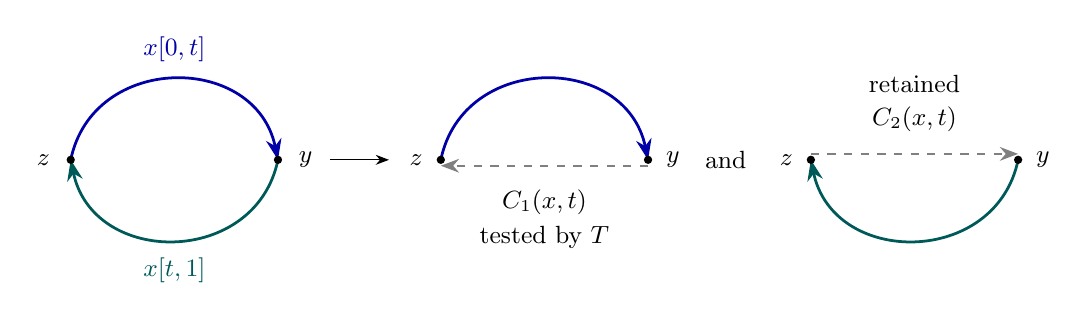
\begin{tikzpicture}[x=.94cm,y=.94cm,>=Stealth,
  every node/.style={font=\small},
  first arc/.style={blue!65!black,line width=1pt},
  second arc/.style={teal!70!black,line width=1pt},
  stick/.style={gray,dashed,line width=.8pt}]
  \draw[first arc,->] (0,0) .. controls (.3,1.45) and (2.5,1.45) .. (2.8,0);
  \draw[second arc,->] (2.8,0) .. controls (2.5,-1.45) and (.3,-1.45) .. (0,0);
  \fill (0,0) circle (1.5pt);
  \fill (2.8,0) circle (1.5pt);
  \node[left=4pt] at (0,0) {$z$};
  \node[right=4pt] at (2.8,0) {$y$};
  \node[above=3pt,text=blue!65!black] at (1.4,1.08) {$x[0,t]$};
  \node[below=3pt,text=teal!70!black] at (1.4,-1.08) {$x[t,1]$};
  \draw[->] (3.5,0) -- (4.3,0);
  \draw[first arc,->] (5,0) .. controls (5.3,1.45) and (7.5,1.45) .. (7.8,0);
  \draw[stick,->] (7.8,-.08) -- (5,-.08);
  \fill (5,0) circle (1.5pt);
  \fill (7.8,0) circle (1.5pt);
  \node[left=3pt] at (5,0) {$z$};
  \node[right=3pt] at (7.8,0) {$y$};
  \node at (6.4,-.58) {$C_1(x,t)$};
  \node at (6.4,-1.05) {tested by $T$};
  \node at (8.85,0) {and};
  \draw[stick,->] (10,.08) -- (12.8,.08);
  \draw[second arc,->] (12.8,0) .. controls (12.5,-1.45) and (10.3,-1.45) .. (10,0);
  \fill (10,0) circle (1.5pt);
  \fill (12.8,0) circle (1.5pt);
  \node[left=3pt] at (10,0) {$z$};
  \node[right=3pt] at (12.8,0) {$y$};
  \node at (11.4,.55) {$C_2(x,t)$};
  \node at (11.4,1.02) {retained};
\end{tikzpicture}
\caption{The native cut at $y=x(t)$, with $z=x(0)$. Short round arcs
(dashed) close the prefix and the remaining path. The cut tests the first
loop and retains the second. The drawing separates the nearby endpoints
to show the two arcs.}
\label{fig:native-cut}
\end{figure}


For a normalized $p$-cocycle $T$ vanishing on $\mathcal A_L$, put
$q=n+p-1$ and define on adequate chains
\begin{equation}\label{eq:cj-cut-definition}
 D_Tx=(C_2)_\#\bigl((x\times I)\frown
 U_c(x(0),x(t))\frown T(C_1(x,t))\bigr).
\end{equation}
Pullback notation in this formula is abbreviated; the second cap
is defined on the supported cut tube.
Absolute extensions of the loop coproduct and their Euler-characteristic
boundary correction were studied by Cieliebak, Hingston and
Oancea~\cite[Section~8.1]{CieliebakHingstonOancea2023}.
Their odd-sphere calculation also exhibits constant-loop output terms
\cite[Proposition~8.3 and Remark~8.4]{CieliebakHingstonOancea2023}.
The filtered comparison for the cut defined here is proved below.

For joining, choose an arbitrarily small radius $\eta_j$ and a
normalized diagonal Thom cocycle $U_j$ relative to $F_{\eta_j}$.
For close $z,z'$, let $J_{z,z'}$ be the shortest plane rotation
taking $z$ to $z'$, and the identity at equality.  The rotations
$J_{z,z'}^u$, $-1\le u\le1$, depend smoothly on the two points
and converge smoothly to the identity as the points approach.
Their $g$-length distortion is at most $1+\kappa$, with
$\kappa\to0$ as $\eta_j\to0$.  Define
\begin{equation}\label{eq:cj-join-definition}
 \mu(x,y)=\bigl((J_{x(0),y(0)}x)\#y\bigr)_\#
 \bigl((x\times y)\frown U_j(x(0),y(0))\bigr).
\end{equation}

\begin{lemma}[Boundary and length properties]\label{lem:cj-operations}
The cut has degree $-q$, takes absolute cycles to absolute cycles,
and preserves global null-homology.  For a cycle in $\mathcal A_a$ it is
supported in
\begin{equation}\label{eq:cj-cut-bound}
 \mathcal A_{a-L+1}.
\end{equation}
The same cut estimate holds on finite fillings.  The join has degree
$-n$ and satisfies the product boundary formula.  On any prescribed
finite collection of chains and fillings its radius can be chosen
so that its output length is less than the sum of the two input
length bounds plus $1$.  All these statements are compatible with
the refinement comparisons above.

If $c$ is a fundamental cycle of constant loops, then
\begin{equation}\label{eq:cj-chain-unit}
 \mu(c,x)\simeq x\quad\text{in }\mathcal A_a
\end{equation}
for every cycle $x$ in $\mathcal A_a$.
\end{lemma}

\begin{proof}
The cut degree is $1-n-p=-q$.  The cap boundary formula applies
by Lemma~\ref{lem:cj-small-chains}; its time-end terms vanish
because $(x(0),x(t))$ is exactly diagonal at $t=0,1$.  Applying
the same construction to a finite filling proves null-homology
preservation.  On a surviving parent the tested first loop has
length at least $L-\varepsilon$, while
\[
 \ell(C_1(x,t))+\ell(C_2(x,t))
 \le\ell(x)+2\varepsilon.
\]
This gives \eqref{eq:cj-cut-bound}.  If its upper level is
nonpositive, no term survives.  The join boundary formula uses
the closed cocycle $U_j$.  Its output length is at most
$(1+\kappa)\ell(x)+\ell(y)$, and $\eta_j$ may be chosen
after all finite length bounds have been specified.

For the unit, consider a shuffle of $c\times x$.  A constant-factor
step remaining after the $n$-cap makes the output degenerate:
the rotated constant is exactly $x(0)$, so the output is independent
of that factor.  The remaining terms have all $n$ constant-factor
steps first.  Their coefficient is the Thom evaluation on
$[M]\times\{x(0)\}$, at the initial parameter vertex of the
$x$-simplex, and equals one.  Thus the output is a constant half
followed by $x$.  Removing the waiting half by reparametrization
gives \eqref{eq:cj-chain-unit} without changing length.
\end{proof}

\subsection{Interchanging which factor is cut}

\begin{theorem}[Filtered interchange]\label{thm:filtered-interchange}
Let $T$ be a normalized cocycle of degree $p\ge1$ vanishing on
$\mathcal A_L$, where $L>0$, and put $q=n+p-1$.  Let $x$ and $y$ be
arbitrary absolute cycles of respective degrees $j,N$ with
\[
 j>n+p,\qquad N>n+p,
\]
supported in $\mathcal A_a$ and $\mathcal A_b$.  With sufficiently small join radius
and adequate refinements,
\begin{equation}\label{eq:cj-interchange}
 \mu(D_Tx,y)\simeq\mu(D_Ty,x)
 \quad\text{in }\mathcal A_{a+b-L+c_{\rm cj}},\qquad c_{\rm cj}=4.
\end{equation}
Both sides have degree $j+N-q-n$.  The constant $c_{\rm cj}$
is independent of both degrees, the cocycle, and all length bounds.
The join radius may be chosen for any additional prescribed finite
collection of fillings without changing this constant.
\end{theorem}

\begin{proof}
Write $J=J_{x(0),y(0)}$ and $Z=(Jx)\#y$.  On
$x\times I_s\times y$, first cap with
$\sigma=U_j(x(0),y(0))$, then with
$U_c(Z(0),Z(s))$, then with $T(C_1(Z,s))$, and output
$C_2(Z,s)$.  Call this cycle $P(x,y)$.  Its time endpoints
vanish by \eqref{eq:cj-diagonal-cocycle}.  We prove
\begin{equation}\label{eq:cj-three-comparisons}
 \mu(D_Tx,y)\simeq P(x,y)\simeq P(y,x)
                   \simeq\mu(D_Ty,x).
\end{equation}
All homologies will have the bound in \eqref{eq:cj-interchange}.

\paragraph{The second half vanishes.}
Split $I_s$ at $1/2$.  At the seam $Z(1/2)=Z(0)$, so each
piece is separately a cycle after capping.  For $s\ge1/2$, both
the cut evaluation and the second-cut output depend only on
$(y,s)$.  A shuffle contains $j$ steps from $x$.  Its join face
uses at most $n$ of them, and its $T$-face at most $p$.
Since $j>n+p$, another such step belongs either to the cut Thom
face or to the retained output face.  In the first case the
normalized Thom evaluation is zero; in the second the output
simplex is degenerate.  In fact projection drops the unused
$x$-step, and the output factors through the corresponding
standard degeneracy map.  Deleting a repeated projected vertex
uses a face of the original simplex, so this factorization stays
within the cut domain.  The second-half cycle therefore bounds
in its image sublevel.

\paragraph{The first half gives the native cut.}
Put $t=2s$ on the first half.  The first cut is exactly
$JC_1(x,t)$.  The second cut consists of an arc, the rotated
$x$-tail and $y$, with respective durations
\[
 \frac12,\qquad\frac{1-t}{2(2-t)},\qquad\frac1{2(2-t)}.
\]
Interpolate them linearly to $1/4,1/4,1/2$.  The result is
$(JC_2(x,t))\#y$.  Length is unchanged, and continuity at
$t=1$ follows because the shrinking tail contributes at most
a fixed multiple of $\int_t^1|x'|^2$ to the energy.

Keep this output fixed and move the cut evaluation and tested
first loop from those of $Jx$ to those of $J^u x$, with $u$
decreasing from $1$ to $0$.  Cross with this parameter before
capping.  Round rotations preserve the cut distance, so all
surviving parents support the fixed output throughout.  The cap
boundary formula gives a homology: it requires continuous
supported maps, not an identity between the fixed output and an
intermediate tested cut.  Its time endpoints remain diagonal.
Small rotation distortion keeps the first-cut plus output length
within a fixed small error of $\ell(x)+\ell(y)$.

At $u=0$ put
\[
 \gamma=U_c(x(0),x(t))\smile T(C_1(x,t)),
\]
using extension by zero as in Lemma~\ref{lem:cj-small-chains}.
This normalized cochain has degree $n+p$ and is independent of
$y$.  Impose the native cut smallness even before the join cap.
We may then commute $\sigma$ and $\gamma$ using
\begin{equation}\label{eq:cj-cup-one}
 \delta(\sigma\smile_1\gamma)
 =\sigma\smile\gamma+\gamma\smile\sigma
       +\sigma\smile_1\delta\gamma.
\end{equation}
For completeness, if the degrees of cochains $u,v$ are $r,s$,
their mod-two cup-one on a simplex of dimension $r+s-1$ is
\[
 \sum_{i=0}^{r-1}
 u[0,\ldots,i,i+s,\ldots,r+s-1]\,
 v[i,\ldots,i+s].
\]
The coboundary formula follows by pairing deletions outside and
inside the block; the shared-end deletions cancel in adjacent
summands except for the two outer cups.  This gives
\eqref{eq:cj-cup-one} since $\delta\sigma=0$.

Lemma~\ref{lem:cj-small-chains} makes $\delta\gamma$ zero
on every block involved, including all extension-by-zero terms.
Each nonzero summand of the primitive has a join face and a
cut/test block.  Its parent is therefore in both tubes and has
high first-cut length.  On either time endpoint the cut part of
every $\gamma$-face vanishes.  Capping with the primitive and
pushing to the fixed output supplies the required homology
between the two cap orders.

With $\gamma$ first, a $y$-step in its front face gives a
degenerate evaluation.  The surviving shuffles start with
$n+p$ steps from $x\times I$.  Their suffixes are exactly
the shuffles of the retained cut face with $y$.  The native
second cut starts at $x(0)$, so the remaining join cap and
output are precisely those of $\mu(D_Tx,y)$.  Common factor
refinements compare any independently chosen join subdivision.
This proves the first comparison in
\eqref{eq:cj-three-comparisons}.

\paragraph{Symmetry of the joined cut.}
Keep the cut interval whole during the following homotopies.
Rotate the entire loop by $J^{-u}$, obtaining
\[
 (J^{1-u}x)\#(J^{-u}y),\qquad 0\le u\le1.
\]
Then translate the circle parameter of $x\#(J^{-1}y)$
through half a period, ending at $(J^{-1}y)\#x$.
Translation is jointly continuous in $H^1$ and preserves length.
At every stage the evaluations at cut times zero and one are
diagonal.  An intermediate half-time seam need not be diagonal;
any seam terms cancel because we use the full interval.

The swapped join cochain represents the same Thom class relative
to $F_{\eta_j}$, and hence differs from $\sigma$ by the
coboundary of a cochain relative to that far set.  A nonzero
face of this primitive forces its whole adequate parent into
the join tube.  Cap with the primitive followed by the cut and
test cochains and use the boundary formula; the cut kills the
time endpoints.  Shuffle symmetry now identifies the result
with $P(y,x)$.  Repeating the first-half argument in the
opposite order proves the last comparison in
\eqref{eq:cj-three-comparisons}; the second half vanishes
because $N>n+p$.

\paragraph{One length bound for all these homologies.}
Choose the join radius so that each partial rotation changes
the length of every path with the prescribed finite bounds by
less than $\varepsilon$.  This is possible after including
the bounds for any additional finite fillings.  In the whole-loop
homotopies a surviving test saves at least $L-\varepsilon$
from the common joined length, at a cost of two short arcs and
small rotations.  In the first-half homotopy with fixed output,
compare the tested $J^u C_1$ with $C_1$; each differs in length
by less than $\varepsilon$.  Together with the two cut arcs
and the output rotation this gives a cost less than
$8\varepsilon$.  Timing changes preserve length.  The cup-one
and primitive comparisons satisfy the same bound by whole-parent
support and oscillation.  Thus each individual homology lies
already below $a+b-L+1$ after sufficiently small choices.
Their sum, together with the image-preserving refinement and
normalization homologies, satisfies the generous common bound
$a+b-L+4$.  The number of chain terms does not add lengths:
the support of a sum is contained in the union of their supports.
Neither a larger degree nor a finer subdivision traverses an
additional long loop.  This proves the claimed uniformity.
\end{proof}

\subsection{Relative scalar comparison and the absolute unit}

The remaining identification uses the established singular models
of the two string-topology products.  We state the scalar comparison
separately because it does not determine constant-loop output
components.

\begin{lemma}[Comparison with the string-topology products]
\label{lem:cj-public-comparison}
The join $\mu$ induces $\bullet$ on ordinary homology.
If $T$ represents a relative class $[T]\in H^p(\Lambda,M)$
and $b$ is a normalized relative cocycle of degree $r$, then
for every absolute cycle $z$ of degree $p+r+n-1$,
\begin{equation}\label{eq:cj-scalar-comparison}
 \langle b,D_Tz\rangle
   =\langle[T]\circledast[b],[z]\rangle.
\end{equation}
Here the brackets on the right also denote the image of $z$ in
relative homology.
\end{lemma}

\begin{proof}
Hingston--Wahl give singular chain models on $H^1$ loops by
capping with the evaluation pullback of a diagonal Thom cocycle,
then adding short arcs and concatenating or cutting
\cite[Theorem~A, Definitions~1.2 and~1.4]{HingstonWahl2023}.
The dual relative operation is the Goresky--Hingston product
\cite[Theorem~2.13]{HingstonWahl2023}; all sign differences
disappear over $\kk$.  We use these models with the auxiliary
round metric and compare the actual maps and cochains.
Choose their support radius to equal ours and their map domain to
contain our larger tube; both choices can be made within their
injectivity-radius requirement.

For joining, partially rotate the first input by $J^u$ and
apply their short-arc retraction, whose values have equal starts
throughout.
Writing $z=x(0)$ and $z'=y(0)$, the residual mismatch satisfies
$d_{\rm rd}(J^u z,z')=(1-u)d_{\rm rd}(z,z')$,
so all inputs remain in its domain.
At $u=0$ this is their retraction; at $u=1$ the inputs already
have equal starts, so their retraction is the identity and gives
our rotation retraction.  This is a homotopy inside equal-start
pairs.  Interpolate their energy-optimal concatenation times to
halves.  For path pieces of square-root energies $P,Q$, the
optimal time for the first piece is $P/(P+Q)$; during this
interpolation its energy contribution is bounded by
\[
 \max\{2P^2,P(P+Q)\}.
\]
This tends to zero if that piece collapses.  The other piece is
handled in the same way, and if both collapse both contributions
vanish.  Thus the timing homotopy is continuous also at constant
pieces.

For cutting, their short-arc retraction followed by cutting gives
exactly the two paths in \eqref{eq:cj-cut-maps}, with optimal
instead of half timings.  The same interpolation compares them.
At either time endpoint one of the two paths remains constant.
Pairing with $T$ and $b$ evaluates on $z\times I$ the cochain
\[
 U_c(x(0),x(t))\smile\chi,\qquad
 \chi=T(C_1(x,t))\smile b(C_2(x,t)).
\]
Both tests are relative to constants.  Hence $\chi$ vanishes
at $t=0$ through its first factor and at $t=1$ through its
second factor.

Replace $U_c$ by the reduced ordinary Thom representative used
in that model.  They differ by a coboundary relative to the
far set.  Although its primitive need not vanish on the diagonal,
all of its time-end contributions are multiplied by $\chi$
and vanish.  If a cap convention reverses the cup order, the
cup-one formula supplies the comparison.  On a small simplex in
the tube, $\chi$ is a closed pullback; on a simplex in the
far set, every face of the accompanying Thom cochain or relative
primitive vanishes.  Thus extension-by-zero errors contribute
nothing, exactly as in Lemma~\ref{lem:cj-small-chains}.
The same argument permits replacement of either relative test
by a cohomologous representative.  Join Thom representatives
are compared in the same way, without interval-end terms.

Finally the Alexander--Whitney map in the coproduct evaluates
$T\otimes b$ as the displayed cup of the two pullbacks.
Their small-chain replacement and our refined products
represent the same relative chain class: both are homologous
to the input, and small-chain inclusion is a quasi-isomorphism,
also relative to the time ends, by subdivision.  This proves
\eqref{eq:cj-scalar-comparison} and the asserted join
identification.  The argument compares two relative tests;
it makes no assertion about a canonical absolute extension of
the coproduct.
\end{proof}

\begin{proposition}[The cut of the power is the absolute unit]
\label{prop:absolute-unit}
For the choices $S,T,l,L$ in \eqref{eq:cj-thresholds},
\begin{equation}\label{eq:cj-absolute-unit}
 [D_TS]=[M]\quad\text{in }H_n(\Lambda).
\end{equation}
Moreover $D_TS$ is supported in $\mathcal A_{l-L+1}$, and there is a
constant $B$ independent of $m$ such that it is homologous to a
fundamental constant-loop cycle in $\mathcal A_B$.
\end{proposition}

\begin{proof}
Represent $\Theta^{\bullet(m+1)}$ by a finite cycle $z$.
Its cut has degree
$n+2(m+1)d-q=3n-2$.  Lemma~\ref{lem:cj-public-comparison},
commutativity of the relative product over $\kk$, and
\eqref{eq:cj-power-pairing} give
$\langle\theta,D_Tz\rangle=1$.  The rank-one calculation
therefore yields $[D_Tz]=\Theta$.

Both $|z|$ and $|S|=n+q$ exceed $n+p=q+1$.
Apply Theorem~\ref{thm:filtered-interchange} to these cycles,
now forgetting the finite output length bound.  Using the join
identification,
\[
 0\ne\Theta^{\bullet(m+1)}
   =[\mu(D_Tz,S)]=[\mu(D_TS,z)].
\]
If $D_TS$ were null-homologous, its join with $z$ would bound,
by Lemma~\ref{lem:cj-operations}.  Thus $D_TS\ne0$ in
$H_n(\Lambda)=\kk[M]$, proving \eqref{eq:cj-absolute-unit}.
This determines the absolute constant component by interchange
and nonvanishing, rather than by the relative scalar test alone.

The cut bound gives support in $\mathcal A_{l-L+1}$.  Its difference
from a constant fundamental cycle is globally null in degree
$n$; Proposition~\ref{prop:fixed-degree-death} fills that
difference in $\mathcal A_{l-L+1+D_n}$.  By
\eqref{eq:cj-fixed-difference}, this is one fixed level $B$.
\end{proof}

The canonical absolute coproduct of
\cite[Theorem~B]{HingstonWahl2023} removes evaluation components;
the cut used here retains the component determined in
Proposition~\ref{prop:absolute-unit}.  The comparison proved
above is specific to this cut and its degree range.  It is not
an invocation of a general Frobenius identity; the canonical
extension fails such an identity
\cite[Remark~4.14]{HingstonWahl2023}.

We have obtained three compatible pieces of information: a cut
which lowers degree and saves length, an interchange homology
with fixed length cost, and a bounded-length correction of
$D_TS$ to the unit.  The next section combines them with
fixed-degree filling to remove the dependence of the filling
increment on the homological degree.

\section{One filling increment in every degree}\label{sec:ordinary}

We combine fixed-degree shortening with the filtered cut--join identity.
The cut removes a degree-dependent amount of length, while its join with
a sphere power restores that length up to one fixed difference.  The
result is a filling increment independent of both degree and level.

\begin{theorem}[Uniform ordinary death]\label{thm:ordinary-death}
For every smooth Riemannian metric on $S^n$, $n\ge3$, there is a constant
$D>0$ such that, for every integer $j\ge0$ and every real $a>0$,
\begin{align}
 \ker\bigl(H_j(X_a)\longrightarrow H_j(\Lambda)\bigr)
 &\subseteq
 \ker\bigl(H_j(X_a)\longrightarrow H_j(X_{a+D})\bigr),
 \label{eq:ordinary-absolute}\\
 \ker\bigl(H_j(X_a,M)\longrightarrow H_j(\Lambda,M)\bigr)
 &\subseteq
 \ker\bigl(H_j(X_a,M)\longrightarrow H_j(X_{a+D},M)\bigr).
 \label{eq:ordinary-relative}
\end{align}
The same constant works at regular and nonregular levels.  No assumption
on the number of prime geodesic images is required.
\end{theorem}

\begin{proof}
We first prove the absolute assertion for the length filtration
$\mathcal A_a$, then pass to square-root energy and to the relative pair.

\paragraph{Choosing the degree reduction.}
Let $d=n-1$ and let $\alpha,C_H$ be the constants of
Proposition~\ref{prop:sphere-powers}.  For sufficiently large $j$ put
\begin{equation}\label{eq:ordinary-degrees}
 m=\left\lfloor\frac{j-2}{2d}\right\rfloor,
 \qquad q=2md,\qquad p=q-d,\qquad N=n+q.
\end{equation}
Then
\begin{equation}\label{eq:ordinary-remainder}
 2\le r:=j-q\le2d+1=2n-1,
 \qquad j>q+1=n+p,
 \qquad N>n+p.
\end{equation}
Choose an integer $J>2n$ so large that, whenever $j\ge J$, these choices
have $m\ge1$, $p>n+1$, and $L>0$ in
\eqref{eq:cj-thresholds}.  Take $S,T,l,L$ as in that equation.  Write
\begin{equation}\label{eq:ordinary-gap}
 C_{\mathrm{gap}}=l-L
   =\frac{2n-1+2C_H}{\alpha}+4,
 \qquad
 D_* =\max_{0\le s<J}D_s,
\end{equation}
where $D_s$ is furnished by Proposition~\ref{prop:fixed-degree-death}.
All the remainder degrees in \eqref{eq:ordinary-remainder}, and the
degree $n$, occur in this finite maximum.

\paragraph{Filling a high-degree null cycle.}
Let $x$ be a finite globally null $j$-cycle in $\mathcal A_a$, with
$j\ge J$.  Its cut $D_Tx$ is a globally null $r$-cycle in
$\mathcal A_{a-L+1}$ by Lemma~\ref{lem:cj-operations}.
If $a-L+1>0$, Proposition~\ref{prop:fixed-degree-death} gives a chain
$W$ such that
\[
 \partial W=D_Tx,
 \qquad\operatorname{supp}W\subset\mathcal A_{a-L+1+D_r}.
\]
If $a-L+1\le0$, the cut has no surviving term and we take $W=0$.

Fix a fundamental constant-loop cycle $c$.  By
Proposition~\ref{prop:absolute-unit}, the cycle $D_TS-c$ is globally
null in degree $n$ and is supported in
$\mathcal A_{C_{\mathrm{gap}}+1}$.  Fixed-degree filling gives a chain
$V$ with
\begin{equation}\label{eq:ordinary-correction}
 \partial V=D_TS-c,
 \qquad
 \operatorname{supp}V\subset
 \mathcal A_{C_{\mathrm{gap}}+1+D_n}.
\end{equation}
This length bound is independent of $j$, although the chain $V$ itself
may depend on the chosen power.

Choose the join radius after these finite length bounds have been
specified.  Lemma~\ref{lem:cj-operations} and
Theorem~\ref{thm:filtered-interchange} permit one choice for the
interchange homology and both joined fillings.  Refinement comparisons
are included in the same bounds.  The relevant chains have the following
supports:
\begin{align}
 \mu(W,S)&\text{ lies in }
   \mathcal A_{a+C_{\mathrm{gap}}+D_*+2},
   \label{eq:ordinary-joined-filling}\\
 \mu(V,x)&\text{ lies in }
   \mathcal A_{a+C_{\mathrm{gap}}+D_*+2}.
   \label{eq:ordinary-joined-correction}
\end{align}
The first assertion is omitted when $W=0$; otherwise it follows by
adding the input bounds $a-L+1+D_r$ and $l$ and the join allowance $1$.
The second follows from \eqref{eq:ordinary-correction} in the same way.
Both chains have degree $j+1$.

The degree inequalities \eqref{eq:ordinary-remainder} are precisely
the two hypotheses needed for the interchange homology.  It gives
\[
 \mu(D_Tx,S)\simeq\mu(D_TS,x)
 \quad\text{in }\mathcal A_{a+C_{\mathrm{gap}}+4}.
\]
The chain $\mu(W,S)$ has boundary $\mu(D_Tx,S)$, while
$\mu(V,x)$ has boundary
$\mu(D_TS,x)-\mu(c,x)$.  Finally
\eqref{eq:cj-chain-unit} joins $\mu(c,x)$ to $x$ in
$\mathcal A_a$.  Adding these chains and the interchange homology
therefore fills $x$.

Thus one permissible length increment is
\begin{equation}\label{eq:ordinary-D}
 D=C_{\mathrm{gap}}+D_*+6.
\end{equation}
It exceeds every bound just used.  For $j<J$, the conclusion follows
directly from Proposition~\ref{prop:fixed-degree-death}, since
$D_j\le D_*<D$.  We have proved that every globally null finite cycle
in $\mathcal A_a$, in any degree, fills in $\mathcal A_{a+D}$.
The constants in \eqref{eq:ordinary-D} depend only on the metric and
$n$, and every construction used above is independent of a finite-prime
hypothesis.

\paragraph{Returning to square-root energy.}
A cycle $x$ in $X_a$ is in $\mathcal A_a$ because $\ell\le F$.
Fill it by the length assertion and apply $\Psi_1$ to that filling.
Lemma~\ref{lem:arclength} gives $F(\Psi_1\gamma)=\ell(\gamma)$, so
the new filling lies in $X_{a+D}$ and has boundary $\Psi_1x$.
The normalization prism from $x$ to $\Psi_1x$ lies entirely in $X_a$
by \eqref{eq:shortening-energy}.  Adding this prism proves
\eqref{eq:ordinary-absolute} with the same $D$.  Strict sublevel
inequalities are preserved throughout; no approximation by regular
levels is involved.

\paragraph{Passing to constants-relative homology.}
Let $i:M\to\Lambda$ include constants and let
$\ev_0:\Lambda\to M$ be evaluation at zero.  Since
$\ev_0\circ i=\operatorname{id}_M$, the chain map
\[
 P=\operatorname{id}-i_\#(\ev_0)_\#
\]
annihilates $C_*(M)$ and preserves $C_*(X_a)$ for every $a>0$.
If $z$ represents a relative cycle in $(X_a,M)$, then
$\partial z\in C_*(M)$, so $Pz$ is an absolute cycle representing
the same relative class.  If $z$ is globally null relative to $M$,
there are finite chains $U$ in $\Lambda$ and $c'$ in $M$ with
$\partial U=z+c'$.  Applying $P$ gives $\partial(PU)=Pz$.
Hence $Pz$ is globally null absolutely.  By
\eqref{eq:ordinary-absolute} it fills in $X_{a+D}$, and passage to
the relative chain quotient proves \eqref{eq:ordinary-relative}.
This argument includes degree zero and uses exactly the same increment.
\end{proof}

The restriction $a>0$ ensures that the constant loops belong to the
relative pair.  For nonpositive $a$ the open absolute sublevel is empty.
Theorem~\ref{thm:ordinary-death} supplies the degree-uniform control of
ordinary transient classes needed for the reflection-equivariant argument
below.

\section{Global equivariant classes}
\label{sec:equivariant}

We now compute the global reflection cohomology and construct the
full-group classes needed in the doubling argument.
The computation uses a round metric only to filter the loop space;
the resulting classes belong to the same global groups for every
metric.  The distinction between odd and even round stages will be
essential.  It is independent of the parity of the sphere dimension.

\subsection{Natural Gysin sequences}

Let \(w\in H^1(BG;\kk)\) and \(U\in H^2(BG;\kk)\) be the
Stiefel--Whitney classes of the standard two-dimensional representation
of \(G=O(2)\).  We use the same letter \(w\) for its restrictions.
Let \(v\in H^1(BK;\kk)\) be the character which is nontrivial on
\(\tau\) and trivial on \(R\).  Then
\begin{equation}
 H^*(BG;\kk)=\kk[w,U],\qquad
 H^*(BK;\kk)=\kk[v,w],\qquad
 \res_K U=v(v+w).
 \label{eqv:coefficient-rings}
\end{equation}
Indeed, the standard plane restricts to the two characters \(v\) and
\(v+w\).  Its projectivization over \(BG\) is \(BK\), so the
projective-bundle formula makes restriction injective
\cite[Section~3.1, pp.~78--79]{HatcherVBKT2017}.  Conjugation
in \(G\) interchanges the two coordinate lines of \(K\), whereas inner
conjugation acts trivially on \(H^*(BG)\).  The image is consequently
contained in the symmetric polynomials in \(v,v+w\).  It contains their
sum \(w\) and product \(U\), which generate that symmetric polynomial
ring.  This proves \eqref{eqv:coefficient-rings}.

For an \(H\)-pair \((Y,A)\), write \(H_H^*(Y,A)\) for its Borel
cohomology.  These groups are zero in negative degrees.

\begin{proposition}[Natural Gysin sequences]
\label{prop:gysin}
For every \(G\)-pair \((Y,A)\), there are natural exact sequences
\begin{align}
 \cdots\longrightarrow H_G^{j-2}(Y,A)
 &\xrightarrow{\,U\,} H_G^j(Y,A)
 \xrightarrow{\res_R} H_R^j(Y,A)
 \xrightarrow{\int} H_G^{j-1}(Y,A)
 \xrightarrow{\,U\,} H_G^{j+1}(Y,A)\longrightarrow\cdots,
 \label{eqv:standard-gysin}\\
 0\longrightarrow H_G^j(Y,A)
 &\xrightarrow{\res_K}H_K^j(Y,A)
 \xrightarrow{\int}H_G^{j-1}(Y,A)
 \longrightarrow0.
 \label{eqv:weight-two-gysin}
\end{align}
For an \(R\)-pair and a \(K\)-pair, respectively, the sign-line
sequences are
\begin{align}
 \cdots\longrightarrow H_R^{j-1}(Y,A)
 &\xrightarrow{\,w\,}H_R^j(Y,A)
 \longrightarrow H^j(Y,A)
 \longrightarrow H_R^j(Y,A)
 \xrightarrow{\,w\,}H_R^{j+1}(Y,A)\longrightarrow\cdots,
 \label{eqv:reflection-gysin}\\
 \cdots\longrightarrow H_K^{j-1}(Y,A)
 &\xrightarrow{\,v\,}H_K^j(Y,A)
 \longrightarrow H_R^j(Y,A)
 \longrightarrow H_K^j(Y,A)
 \xrightarrow{\,v\,}H_K^{j+1}(Y,A)\longrightarrow\cdots.
 \label{eqv:half-shift-gysin}
\end{align}
The maps commute with maps of pairs and subgroup restriction wherever
the latter applies, and satisfy the projection formula for absolute
base classes.
\end{proposition}

\begin{proof}
For a real rank-\(r\) representation of \(H\), its associated bundle
over \(Y_H\) restricts to a bundle over \(A_H\).
Suppose that its unit sphere is \(H/H'\).
The sphere-bundle pair is then the Borel pair for \(H'\).
The relative Thom sequence gives
\begin{equation}
 \cdots\longrightarrow H_H^{j-r}(Y,A)
 \xrightarrow{\,w_r\,}H_H^j(Y,A)
 \longrightarrow H_{H'}^j(Y,A)
 \xrightarrow{\int}H_H^{j-r+1}(Y,A)\longrightarrow\cdots.
 \label{eqv:general-gysin}
\end{equation}

Here is a cochain construction that also justifies
\eqref{eqv:general-gysin} when the inclusion \(A_H\subset Y_H\) is not
a cofibration.  For a vector bundle over \(Z\supset A_0\), let \(D,S\)
denote its disk and sphere bundles, and let \(D_{A_0},S_{A_0}\)
be their restrictions.  In the singular chain complex of \(D\), put
\[
 \mathcal L=C_*(S)+C_*(D_{A_0}).
\]
The two summands intersect in \(C_*(S_{A_0})\), since singular chains
have the singular simplices as a basis.  Restriction of cochains gives
degreewise exact sequences
\begin{align*}
 0&\longrightarrow\operatorname{Ann}\mathcal L
 \longrightarrow C^*(D,S)
 \longrightarrow C^*(D_{A_0},S_{A_0})\longrightarrow0,\\
 0&\longrightarrow\operatorname{Ann}\mathcal L
 \longrightarrow C^*(D,D_{A_0})
 \longrightarrow C^*(S,S_{A_0})\longrightarrow0.
\end{align*}
Surjectivity follows by extending linear functionals on chain
subspaces.  Cup with a Thom cocycle sends a relative base cochain into
\(\operatorname{Ann}\mathcal L\): on \(S\) the Thom factor vanishes,
and on \(D_{A_0}\) the base factor vanishes.
Comparison of the first sequence with the base-pair sequence, using
the absolute Thom isomorphisms, proves
\[
 H^{j-r}(Z,A_0)\cong H^j(\operatorname{Ann}\mathcal L).
\]
The second sequence and the disk contraction give
\eqref{eqv:general-gysin}.  The map back to the base is cup with the
zero-section pullback of the Thom class, namely \(w_r\).
Pullback of Thom classes gives naturality and the projection formula.
The absolute Thom isomorphism used here is the ordinary mod-two
one \cite[Section~3.2, pp.~88--89]{HatcherVBKT2017};
for a general base it follows by pulling back to its singular
CW replacement and using the disk and sphere fibrations.
This argument uses the sum of two chain subspaces and does not require
an excision assertion for their union.

The standard \(G\)-plane has sphere stabilizer \(R\) and Euler class
\(U\), proving \eqref{eqv:standard-gysin}.
Let \(\rho_2\) be the representation that doubles rotation angles and
sends the chosen reflection to \(\operatorname{diag}(1,-1)\).
Its sphere stabilizer is \(K\).  On \(K\) it has a fixed line, so its
Euler class restricts to zero.  The injectivity in
\eqref{eqv:coefficient-rings} makes that Euler class zero already on
\(BG\), giving \eqref{eqv:weight-two-gysin}.
Finally, the sign representations with kernels \(1\subset R\) and
\(R\subset K\) have Euler classes \(w\) and \(v\), respectively.
\end{proof}

\subsection{The classes to be constructed}

Evaluation at zero is \(R\)-invariant.  If
\(\sigma\in H^n(S^n;\kk)\) is the nonzero class, set
\[
 e=\ev_0^*\sigma\in H_R^n(\Lambda;\kk).
\]
In particular \(e^2=0\).  Recall that \(d=n-1\), and put
\[
 a_m=(2m-1)d\qquad(m\ge1).
\]

\begin{theorem}[Global generators and full-group lifts]
\label{thm:global-generators}
For \(n\ge3\), there are classes
\[
 X_m\in B_\infty^{a_m}=H_R^{a_m}(\Lambda,M),\qquad m\ge1,
\]
with the following properties.
\begin{enumerate}[label=\textup{(\roman*)}]
\item The classes
\[
 \xi_{m,k}=w^kX_m,\qquad
 \eta_{m,k}=e\,w^kX_m,
 \qquad m\ge1,\quad 0\le k\le d,
\]
form a graded \(\kk\)-basis of \(B_\infty\).  Their degrees are
\[
 |\xi_{m,k}|=a_m+k,\qquad
 |\eta_{m,k}|=a_m+n+k.
\]
We call the \(\xi_{m,k}\) the \emph{bottoms} and the \(\eta_{m,k}\)
the \emph{tops} at stage \(m\).
Multiplication by \(w^n\) annihilates \(B_\infty\).
\item Every \(X_m\) is the restriction of a class
\(\zeta_m\in H_G^{a_m}(\Lambda,M)\).
If \(m\) is odd, then \(U^n\zeta_m=0\).
If \(m\) is even, there is also a class
\(Y_m\in H_G^{a_m+n}(\Lambda,M)\) with
\(\res_R Y_m=eX_m\).
\item For the round metric, let \(Z_p\) be an open regular sublevel
containing exactly the first \(p\) positive critical manifolds,
and choose \(Z_0\) below the first one.
For \(H=R,G\), every crossing sequence for
\((Z_p,Z_{m_0-1})\), \(p\ge m_0\), is short exact.
A chosen class of the \(m\)-th crossing has a unique extension to
\(H_H^j(\Lambda,Z_{m-1})\) whenever \(j<a_{m+1}\), for
\(H=R,G\).  The lifts in \textup{(ii)} and the classes \(X_m\)
can be obtained from these relative extensions.
\end{enumerate}
\end{theorem}

The top classes in \textup{(ii)} are chosen lifts; they need not be
canonical.  Only their reflection restrictions will be used.
Also, the annihilation statement in \textup{(i)} is relative to
constants.  The absolute constant-loop Borel summand retains its
polynomial \(w\)-tower.

\subsection{Round crossings}

Give \(S^n\) its unit round metric and write \(E_0\) for its energy.
The positive critical values are \(c_m=(2\pi m)^2\).
The critical manifold at \(c_m\) consists of the loops
\begin{equation}
 \gamma_{x,u}(t)=x\cos(2\pi mt)+u\sin(2\pi mt),
 \qquad |x|=|u|=1,\quad x\perp u.
 \label{eqv:round-loops}
\end{equation}
It is \(C_m=STS^n\), the manifold of orthonormal two-frames in
\(\mathbb R^{n+1}\).

\begin{lemma}[Round attachment]
\label{eqv:round-attachment}
The negative bundle of \(C_m\) has rank \(a_m\), and the kernel of the
round Hessian is exactly \(TC_m\).
For every closed subgroup \(H\subset G\), the crossing has a Thom
isomorphism
\begin{equation}
 H_H^j(Z_m,Z_{m-1})\cong H_H^{j-a_m}(C_m).
 \label{eqv:crossing-thom}
\end{equation}
These isomorphisms commute with subgroup restriction and cup by
absolute classes.  The small sublevel \(Z_0\) retracts
\(G\)-equivariantly to \(M\).
\end{lemma}

\begin{proof}
Along \eqref{eqv:round-loops}, put
\[
 e_t=-x\sin(2\pi mt)+u\cos(2\pi mt).
\]
A tangent field is \(a(t)e_t+b(t)\), where
\(b(t)\perp\operatorname{span}\{x,u\}\).
Half the Hessian is
\begin{equation}
 \int_0^1\bigl(|a'|^2+|b'|^2-(2\pi m)^2|b|^2\bigr)\,dt.
 \label{eqv:round-hessian}
\end{equation}
In each of the \(d\) normal directions, the negative Fourier
frequencies are \(|k|<m\).  Their real dimension is \(2m-1\).
The null modes are the two normal modes at frequency \(m\), together
with the constant tangential mode.  They have dimension \(2d+1\)
and are precisely the variations of the frame \((x,u)\).
The nonzero Fourier eigenvalues, divided by the corresponding squared
\(H^1\)-norms, are bounded away from zero.  Thus the Hessian is
invertible on the orthogonal complement of its kernel.
At constants, the Hessian is \(2\int|V'|^2\), positive and invertible
off its constant kernel.

We describe why the resulting attachment respects the full group.
Use the strong metric induced by the Euclidean \(H^1\)-norm.
Each parameter symmetry is a smooth isometry, and the action is
continuous.  Pointwise exponential gives a chart on the Hilbert
normal bundle of the compact manifold \(C_m\), at a uniform small
radius.  In these coordinates Taylor's formula writes the energy
difference as \(\langle A(z,y)y,y\rangle\), with
\(A(z,0)\) an invertible symmetric operator on the normal fiber.
Normalize first by \(|A(z,0)|^{1/2}\), and let
\(J=\operatorname{sign}A(z,0)\).
For the resulting operator \(B\) near \(J\), the norm-convergent
power series \(C=(JB)^{1/2}\) satisfies \(C^*JC=B\).
The change \(y\mapsto C(z,y)y\) is a diffeomorphism after shrinking
the tube.  All these constructions commute with the parameter
isometries.  They give the exact normal form
\begin{equation}
 E_0=c_m-|u_-|^2+|u_+|^2
 \label{eqv:round-normal-form}
\end{equation}
on the negative and positive bundles.

For completeness, the sublevel attachment uses the original Hilbert
space, rather than a polygon model with only finite rotational
symmetry.  Patch a complete normalized descending gradient field to
the split field
\[
 \dot z=0,\qquad \dot u_-=u_-,\qquad \dot u_+=-u_+
\]
inside the normal tube, using an invariant squared-radius cutoff.
Both fields strictly decrease \(E_0\) away from \(C_m\) within the
isolating energy band.
The coordinate derivatives are uniformly bounded in a small tube over
the compact zero section, so the patched field remains bounded.
The ambient strong metric is complete; hence this field is complete.
Palais--Smale and regular-band deformation
(Lemmas~\ref{lem:local-analytic} and~\ref{lem:local-strips})
give a uniform decrease outside any smaller tube in an isolating
energy band.
The flow-lens construction of Lemma~\ref{lem:local-lens}
therefore computes the crossing in that smaller tube.
Use its notation \(X,Y,N,Q\), with lower energy cut \(t_-<c_m\).
In split coordinates, contraction of \(u_+\) decreases both endpoint
energies of a trapped flow segment.  It defines maps \(N\to X\)
taking \(Q\) into \(Y\), even when a contracted point leaves \(N\)
through the lower endpoint.  Via \(N/Q\cong X/Y\), these maps induce
a contraction to the negative disk with its boundary collapsed.
For flow time \(T\), the surviving disk before applying the flow has
radius \(e^{-T}\sqrt{c_m-t_-}\); its boundary flows to the lower cut.
The flow multiplies \(u_-\) by \(e^T\), identifying this disk and
sphere with the usual negative-bundle disk and sphere.
The disk is closed in the lens and meets \(Q\) exactly in its sphere.
These statements remain true after Borel construction.
The disk/sphere quotient consequently embeds in the lens quotient:
the saturation of a closed subset of the disk is that subset,
possibly together with the closed collapse set.
The contraction fixes its image.
The disk/sphere inclusion is a good pair.  This proves
\eqref{eqv:crossing-thom} by the mod-two Thom isomorphism.

All pair maps just used are \(G\)-equivariant.  The negative bundle
carries its actual derivative action; no triviality of that action
is assumed.  Restriction to a subgroup and cup by an absolute class
therefore commute with the attachment isomorphism.
Wider regular cuts give the same assertion by regular-band
deformation.  Finally, sufficiently small energy places a loop in
the positive normal chart of the constants, where contraction of
the normal coordinate proves the last assertion.
\end{proof}

\subsection{Cohomology of the critical manifolds}

Reflection sends \((x,u)\) to \((x,-u)\).
It acts freely on \(C_m\), and
\[
 (C_m)_R\simeq P(TS^n).
\]
The sign line is the tautological line in this projective bundle.
Since \(TS^n\oplus\mathbb R\) is trivial, its positive
Stiefel--Whitney classes vanish.  The projective-bundle formula gives
\begin{equation}
 H_R^*(C_m)=\kk[w,e]/(w^n,e^2).
 \label{eqv:reflection-critical-ring}
\end{equation}
Here \(e\) is pulled back from the first frame vector \(x\).
This computation uses mod-two coefficients also when \(n\) is even.
Write \(x_m\) for the bottom Thom class of the crossing, with the
group understood.  Its subgroup restrictions are the corresponding
bottom classes.
Thus the reflection crossing has basis
\begin{equation}
 w^k x_m,\quad ew^k x_m,\qquad 0\le k\le d,
 \label{eqv:reflection-local-basis}
\end{equation}
with degrees \(a_m+k\) and \(a_m+n+k\).

For \(j\ge1\), let \(\rho_j:G\to O(2)\) multiply rotation angles
by \(j\) and preserve the chosen reflection.
The pullbacks of the two plane classes are
\begin{equation}
 w_1(\rho_j)=w,\qquad w_2(\rho_j)=(j\bmod2)U.
 \label{eqv:weight-classes}
\end{equation}
To check the second identity, restrict to \(BSO(2)\), where a
weight-\(j\) complex line multiplies the first Chern class by \(j\).
The only possible additional degree-two term is a multiple of
\(w^2\); restriction to \(BR\), where the plane has a trivial line,
excludes that term.

\begin{lemma}[Odd and even critical modules]
\label{eqv:critical-modules}
Define homogeneous polynomials \(A_i\in\kk[w,U]\) by
\begin{equation}
 A_0=1,\qquad A_1=w,\qquad
 A_i=wA_{i-1}+UA_{i-2}\quad(i\ge2).
 \label{eqv:grassmann-recurrence}
\end{equation}
If \(m\) is odd, the \(G\)-crossing is generated over
\(\kk[w,U]\) by \(x_m\), and
\begin{equation}
 A_{d+1}x_m=A_{d+2}x_m=0.
 \label{eqv:grassmann-relations}
\end{equation}
If \(m\) is even, multiplication by \(U\) is injective on the
\(G\)-crossing, and that crossing is generated over \(\kk[w,U]\)
by \(x_m\) and a chosen class \(y_m\) of degree \(a_m+n\)
whose reflection restriction is \(ex_m\).
\end{lemma}

\begin{proof}
The \(G\)-action on frames is the right action through \(\rho_m\),
up to the convention for inverse precomposition.
For odd \(m\), the map from the critical Borel space to
\(\mathrm{Gr}_2(\mathbb R^{n+1})\) has fiber the classifying space
of the cyclic group of order \(m\).
Local choices of frames give local trivializations.
That fiber has no positive-degree mod-two cohomology, by transfer,
so the map induces a cohomology isomorphism.
The tautological plane pulls back to the plane of \(\rho_m\);
its classes are \(w,U\) by \eqref{eqv:weight-classes}.

These two classes generate the Grassmann cohomology.
Indeed, projectivize the tautological plane.
On the resulting ordered-line flag space, let \(s,t\) be the first
Stiefel--Whitney classes of its two lines.
Over the Grassmannian, the projective-bundle formula gives a free
module with basis \(1,s\).
Over \(\mathbb{RP}^n\), the same flag space is the projectivization
of the first line's perpendicular bundle, so its ring is generated
by \(s,t\).
Since \(s+t=w\), \(st=U\), and \(s^2=ws+U\), every polynomial
in \(s,t\) reduces to \(P(w,U)+sQ(w,U)\).
Uniqueness of the free-module expansion implies that every class
pulled back from the Grassmannian is a polynomial in \(w,U\).
The complementary bundle has rank \(d\), with total
Stiefel--Whitney class \((1+w+U)^{-1}\).
Its components are the polynomials \(A_i\), proving
\eqref{eqv:grassmann-relations} and the odd-stage assertion.

If \(m\) is even, \(\tau\) acts trivially on the critical manifold.
Consequently
\[
 H_K^*(C_m)=H_R^*(C_m)[v].
\]
The same statement holds for the crossing modules after the Thom
shift, with the actual equivariant negative bundle retained.
The polynomial \(U=v(v+w)\) is monic in \(v\), hence acts injectively
even though the coefficient ring in
\eqref{eqv:reflection-critical-ring} has zero divisors.
The injection in \eqref{eqv:weight-two-gysin} makes \(U\) injective
on the \(G\)-crossing as well.
Sequence \eqref{eqv:standard-gysin} therefore identifies the quotient
of the \(G\)-crossing by \(U\) with the \(R\)-crossing.
Choose a lift \(y_m\) of \(ex_m\); the bottom \(x_m\) already lifts.
Their \(w\)-multiples generate modulo \(U\), by
\eqref{eqv:reflection-local-basis}.
Subtracting such a combination and dividing the remainder by \(U\)
reduces degree by two, so induction from the bottom degree proves
generation.
\end{proof}

\subsection{Collapse on all round intervals}

\begin{lemma}[Interval collapse and supported extensions]
\label{eqv:interval-collapse}
Fix \(m_0\ge1\).
For \(H=R,G\) and \(p\ge m_0\), the crossing sequence is short exact:
\begin{equation}
 0\longrightarrow H_H^j(Z_p,Z_{p-1})
 \longrightarrow H_H^j(Z_p,Z_{m_0-1})
 \longrightarrow H_H^j(Z_{p-1},Z_{m_0-1})
 \longrightarrow0.
 \label{eqv:interval-short-exact}
\end{equation}
Restriction induces an isomorphism
\begin{equation}
 H_H^j(\Lambda,Z_{m-1})
 \longrightarrow H_H^j(Z_m,Z_{m-1})
 \qquad\text{if }j<a_{m+1}.
 \label{eqv:unique-relative-lift}
\end{equation}
\end{lemma}

\begin{proof}
First use \(H=R\), inducting on \(p\).
By \eqref{eqv:reflection-local-basis}, the earlier interval module
is generated over the ambient classes \(w,e\) by chosen extensions
of its bottoms \(x_j\), \(m_0\le j<p\).
The connecting homomorphism sends such a bottom into the new crossing
in degree \(a_j+1<a_p\), where the crossing is zero.
It is linear over \(w,e\), hence vanishes on the whole earlier module.
This proves \eqref{eqv:interval-short-exact} for \(R\), and also
justifies the inductive generation assertion.

For \(G\), Lemma~\ref{eqv:critical-modules} gives the same induction
with the bottom generators and, at even stages \(j\), the chosen
top generators of degree \(a_j+n\).
Bottoms again have zero connecting image.
For a top, the only potentially relevant degree is \(a_j+n+1\).
If \(d>2\), then \(n+1=d+2<2d\), so this degree is less than \(a_p\).
If \(d=2\), equality can occur only when \(j=p-1\) is even.
In this case \(p\) is odd, and the target is its one-dimensional
bottom \(G\)-crossing.
Restriction to the corresponding reflection bottom is injective:
both bottom Thom classes restrict to the nonzero bottom class.
The reflection connecting map has already been proved zero.
Naturality therefore kills the \(G\)-connecting map in this last
case as well.  This proves \eqref{eqv:interval-short-exact} in every
dimension \(n\ge3\).

We pass to the global pair degree by degree.
Every singular chain in the Borel construction is finite and has
bounded round energy, since energy descends to a continuous invariant
function.  Thus
\[
 H_j^H(\Lambda,Z_{m-1})
 =\varinjlim_{p\ge m}H_j^H(Z_p,Z_{m-1}).
\]
Universal coefficients over the field \(\kk\) identify its dual with
the inverse limit of the degree-\(j\) cohomology groups.
The local crossing groups vanish below \(a_p\), which tends to
infinity.  Sequence \eqref{eqv:interval-short-exact} consequently
stabilizes in every degree.
For \(j<a_{m+1}\), no subsequent crossing contributes, proving
\eqref{eqv:unique-relative-lift}.
All limits in this argument are taken in a fixed degree; the total
cohomology module is the graded direct sum.
\end{proof}

Since \(Z_0\) retracts equivariantly to \(M\), the triple exact sequence
identifies \(H_H^*(Z_p,Z_0)\) with \(H_H^*(Z_p,M)\), and likewise
\(H_H^*(\Lambda,Z_0)\) with \(H_H^*(\Lambda,M)\).
Thus the first interval filtration computes precisely the global
groups relative to constants used below.

Choose the relative extension
\[
 \widetilde\zeta_m\in H_G^{a_m}(\Lambda,Z_{m-1})
\]
of the bottom Thom class.
Map it to \(H_G^{a_m}(\Lambda,M)\), and call the resulting class
\(\zeta_m\).
Let \(X_m=\res_R\zeta_m\).
For even \(m\), choose \(y_m\) as in
Lemma~\ref{eqv:critical-modules}.
Since
\begin{equation}
 n=d+1<2d,
 \label{eqv:strict-top-gap}
\end{equation}
it has a unique relative extension in degree \(a_m+n\).
Call its image in \(H_G^*(\Lambda,M)\) \(Y_m\).
Restriction and cup by \(e\) commute with the relative extensions;
both have local value \(ex_m\).
Uniqueness in \eqref{eqv:unique-relative-lift} therefore gives
\begin{equation}
 \res_RY_m=eX_m\qquad(m\ \text{even}).
 \label{eqv:even-top-restriction}
\end{equation}

Similarly, \(w^n\res_R\widetilde\zeta_m\) has local value zero
by \eqref{eqv:reflection-critical-ring}.
Its offset is \(n<2d\), so uniqueness gives
\begin{equation}
 w^nX_m=0.
 \label{eqv:global-w-relation}
\end{equation}
The products \(w^kX_m,ew^kX_m\), \(0\le k\le d\), now form a basis
of \(B_\infty\).
To see independence, restrict a finite relation to the lowest round
stage occurring in it: later classes vanish there, while the
remaining leading terms form the local basis
\eqref{eqv:reflection-local-basis}.
Repeat with successive stages.
For spanning, in each fixed degree the interval short exact sequences
give precisely the sum of the local dimensions, and only finitely
many stages contribute.
Equation \eqref{eqv:global-w-relation} and multiplication by \(e\)
show that \(w^n\) annihilates the entire relative module.

\subsection{Odd-stage torsion}

The remaining full-group relation follows from one integration
calculation.  This will also keep the dimension-three case within
the strict extension range.

\begin{lemma}[Torsion of odd bottoms]
\label{eqv:odd-torsion}
For every odd \(m\) and every \(n\ge3\),
\[
 U^n\zeta_m=0.
\]
When \(n=3\), the supported relative lift also satisfies
\[
 w^3\widetilde\zeta_m=0,\qquad
 U(w^2+U)\widetilde\zeta_m=0.
\]
\end{lemma}

\begin{proof}
The recurrence \eqref{eqv:grassmann-recurrence} implies
\begin{equation}
 A_i^2+A_{i-1}A_{i+1}=U^i\qquad(i\ge1).
 \label{eqv:determinant-identity}
\end{equation}
Indeed, substitution of the recurrence makes the left side for
\(i\ge2\) equal to \(U\) times the left side for \(i-1\);
the initial value is \(w^2+A_2=U\).

At an odd crossing, \eqref{eqv:grassmann-relations} gives
\[
 UA_dx_m=(A_{d+2}+wA_{d+1})x_m=0.
\]
The class \(A_dx_m\) is nonzero: on restriction to \(R\), it becomes
\(w^dx_m\), which is nonzero in
\eqref{eqv:reflection-local-basis}.
The relevant part of the standard-plane Gysin sequence is
\[
 H_R^{a_m+d+1}(Z_m,Z_{m-1})
 \xrightarrow{\int} H_G^{a_m+d}(Z_m,Z_{m-1})
 \xrightarrow{U} H_G^{a_m+d+2}(Z_m,Z_{m-1}).
\]
Its source is one-dimensional, spanned by \(ex_m\).
Since its image contains the nonzero class \(A_dx_m\), exactness
over \(\kk\) forces
\begin{equation}
 \int ex_m=A_dx_m.
 \label{eqv:local-integration}
\end{equation}

Apply the same integration map to
\(e\,\res_R\widetilde\zeta_m\) in the pair
\((\Lambda,Z_{m-1})\).
Naturality and \eqref{eqv:local-integration} identify its restriction
to the crossing with \(A_dx_m\).
Both sides have offset \(d<2d\), so
\eqref{eqv:unique-relative-lift} gives
\[
 \int\bigl(e\,\res_R\widetilde\zeta_m\bigr)
   =A_d\widetilde\zeta_m.
\]
The next map in Gysin is multiplication by \(U\), hence
\begin{equation}
 UA_d\widetilde\zeta_m=0.
 \label{eqv:integrated-relation}
\end{equation}
Also \(A_{d+1}\widetilde\zeta_m=0\), because its local value is zero
and \(d+1<2d\).
Multiplying \eqref{eqv:determinant-identity} at \(i=d\) by
\(U\widetilde\zeta_m\) therefore gives
\[
 U^{d+1}\widetilde\zeta_m
 =UA_d^2\widetilde\zeta_m+
   UA_{d-1}A_{d+1}\widetilde\zeta_m=0.
 \]
Its image in \(H_G^*(\Lambda,M)\) is \(U^n\zeta_m=0\).

For \(n=3\), one has \(d=2\), \(A_2=w^2+U\), and \(A_3=w^3\).
The two intermediate global relations are exactly
\[
 w^3\widetilde\zeta_m=0,\qquad
 U(w^2+U)\widetilde\zeta_m=0.
\]
Their proof used uniqueness only at offsets two and three, both
strictly less than the next-bottom gap four.
It did not extend an offset-four relation across that gap.
\end{proof}

The basis construction, \eqref{eqv:even-top-restriction}, and
Lemma~\ref{eqv:odd-torsion} complete the proof of
Theorem~\ref{thm:global-generators}.
For later use, the degree intervals for the bottom family are
\([a_m,a_m+d]\), and those for the top family are
\([a_m+n,a_m+n+d]\).
Intervals within either family are disjoint, since their starting
degrees differ by \(2d\); a bottom and a top can have the same degree.
Thus restrictions of tops will be counted modulo all restricted
bottoms.
The next sections compare those global restrictions with the extra
classes present at a finite cut.

\section{A finite-cut defect bound}\label{sec:budget}

Throughout this section we assume that there are finitely many prime
geodesic images. Our objective is to compare a sublevel with its
half-translation fixed locus while retaining the information lost by
localization. The comparison has two degrees: the total equivariant
degree upstairs and the degree of a root loop downstairs. An exact-sequence
calculation will bound their discrepancy, summed over all degree cutoffs,
by the number of critical events.

Write
\[
 B_a^l=H_R^l(X_a,M),\qquad
 B_\infty^l=H_R^l(\Lambda,M).
\]
At a regular cut these reflection groups have finite total dimension:
Theorem~\ref{thm:local-control} identifies each reflection crossing with
a finite sum of ordinary one-orientation crossing groups, and there are
only finitely many crossings below a finite cut. All sublevels in the
statements are open. At regular endpoints, the deformations of
Lemmas~\ref{lem:local-strips} and~\ref{lem:local-polygons} identify them, naturally
under inclusion and fixed restriction, with closed regular polygon
models. We use those compact models in the localization argument.

\begin{lemma}[Finite-pair localization]\label{bud:localization}
Let $2a>0$ be regular. Then $a$ is regular, and restriction to the
half-translation fixed locus induces an isomorphism
\[
 H_K^*(X_{2a},M)[v^{-1}]
 \longrightarrow H_K^*(X_{2a}^{\tau},M)[v^{-1}].
\]
It is an actual isomorphism in every sufficiently high degree, with the
threshold allowed to depend on $a$. The same localization assertion
holds for crossing pairs and respects their individual prime labels.

For an ambient crossing at the $m$-th iterate of a prime, its actual
$K$-group has uniformly bounded dimension in every degree, is zero below
$I_m-A$, and maps isomorphically to its stabilized fixed target above
$I_m+A$, after increasing the uniform constant $A$. For odd $m$ that
target is zero; for even $m$ its root labels satisfy
$|l-I_{m/2}|\le A$.
\end{lemma}

\begin{proof}
A critical root doubles to a critical loop, so regularity of $2a$
implies regularity of $a$. Doubling identifies $X_a$ with
$X_{2a}^{\tau}$ as an $R$-space. Since $\tau$ acts trivially there, a
product universal model and the field K\"unneth formula give
\begin{equation}\label{bud:fixed-product}
 H_K^J(X_{2a}^{\tau},M)
 =\bigoplus_{l\le J}v^{J-l}B_a^l.
\end{equation}
The same identification holds for fixed crossing pairs.

Choose a common even polygon model through the cut, and double its
compact regular sublevel along an invariant collar. Denote the resulting
closed smooth $K$-manifold by $\mathcal D$. Inclusion of the original
sublevel and the fold map make its restriction arrow to the fixed locus
a retract of the corresponding arrow for $\mathcal D$. The fixed
submanifold $\mathcal D^\tau$ has an invariant open tubular neighborhood
$O_0$ which retracts equivariantly onto it. The compact complement of
$O_0$ is covered by finitely many invariant open sets $O_1,\ldots,O_s$,
each admitting an equivariant map to $K/H_i$ with $\tau\notin H_i$.
Indeed, use a small stabilizer-invariant neighborhood disjoint from its
translates by other cosets, and then saturate it.

The possible groups $H_i$ are $1$, $R=\langle r\rangle$, and
$\langle\tau r\rangle$.
On each, $U=v(v+w)$ restricts to zero. Thus $U$ lifts to
$H_K^2(\mathcal D,O_i)$. Cup these lifts with a class relative to $O_0$.
The relative cup product for the open cover has target relative to
$\bigcup_{i=0}^sO_i=\mathcal D$, so $U^s$ annihilates
$H_K^*(\mathcal D,O_0)$. The exact sequence of this pair proves
localization at $U$. Passing to the retract proves it on the original
sublevel. The exact sequences for a pair of regular sublevels, and for
the pair relative to $M$, give the corresponding assertions for pairs.

The class $w$ is zero on each ambient local block, because that block
is induced from the $\langle\tau\rangle$-pair of one orientation.
It is therefore nilpotent on each finite-cut relative group by induction
over the crossing exact sequences. The same argument applies to the
fixed reflection groups and to crossing pairs. On these modules
localization at $U$ is equivalent to localization at $v$: after
inverting $v$, the factor $1+w/v$ in $U=v^2(1+w/v)$ is invertible;
after inverting $U$, the element $(v+w)/U$ is an inverse for $v$.

Apply the sign-line Gysin sequence of Proposition~\ref{prop:gysin} to
one orientation of a local block. The total ordinary rank bound and
index support in Theorem~\ref{thm:local-control} imply the claimed
per-degree bound, vanishing below the index window, and that multiplication
by $v$ is an isomorphism above it. The fixed local group has the product
description in \eqref{bud:fixed-product}. Its root support is within a
fixed distance of $I_{m/2}$, and
\[
 |I_m-2I_{m/2}|\le n.
\]
Consequently both source and target have already stabilized above
$I_m+A$, with a uniform enlarged $A$. The localized restriction
isomorphism is then an actual isomorphism there: clear a power of $v$
and invert the intervening, already invertible multiplication maps.
For an odd iterate the fixed block is empty, so its stabilized source
is zero. Labelwise naturality follows from the common full/fixed lens
in Theorem~\ref{thm:local-control}.

Finally, the sign-line Gysin sequence from $K$ to $R$ and the finite
total dimension of $B_{2a}$ make multiplication by $v$ an isomorphism
on the ambient relative group in all sufficiently high degrees.
The fixed group has the same property by \eqref{bud:fixed-product}.
The same clearing argument upgrades localization to actual restriction
in high degrees at this cut.
\end{proof}

For a paired regular cut $(2a,a)$, put
\[
 \mathcal V_a=\bigoplus_l B_a^l,\qquad
 A_J=H_K^J(X_{2a},M).
\]
Dropping the powers $v^{J-l}$ in \eqref{bud:fixed-product} defines the
normalized actual restriction
$\epsilon_J:A_J\to\mathcal V_a$. Set
\[
 E_J=\im\epsilon_J,\qquad t_J=\dim\ker\epsilon_J.
\]
The image $E_J$ lies in labels at most $J$; it need not be graded by
root label, and it need not equal the stabilized target. In these
normalized coordinates, multiplication by $v$ leaves a vector unchanged,
whereas multiplication by $w$ applies the root $w$ to each component and
raises its label by one.

Let $P_j$ denote projection to root labels at most $j$. We record three
defects: the dimension missing from the projected low root degrees,
the dimension of actual-image vectors supported entirely above the cutoff,
and the dimension of actual classes invisible on the fixed locus.
They are, respectively, $D_{j,q}$, $H_{j,J}$, and $t_J$.
The potential also includes the preceding-degree deficit $D_{j,2j-1}$;
this compensates for the degree shift in the connecting homomorphism.
Define
\begin{equation}\label{bud:potential}
 \begin{split}
 D_{j,q}&=\dim P_j\mathcal V_a-\dim P_jE_q,\\
 H_{j,J}&=\dim(E_J\cap\ker P_j),\qquad J=2j,\\
 \Phi_j(a)&=D_{j,2j}+D_{j,2j-1}+H_{j,2j}+t_{2j},
 \qquad j\ge1.
 \end{split}
\end{equation}
All four terms are nonnegative. Lemma~\ref{bud:localization} shows that
they vanish for sufficiently large $j$ at any fixed cut.

\begin{theorem}[Finite-cut defect bound]\label{thm:finite-cut-budget}
There is a constant $C$ such that, whenever $2a>0$ is regular,
\begin{equation}\label{bud:linear-budget}
 \sum_{j\ge1}\Phi_j(a)\le C(1+a).
\end{equation}
\end{theorem}

\begin{proof}
Grow the ambient cut through its critical events, using primes for the
groups just after an event. Let $C^q$ be its actual local $K$-group and
$\mathcal W$ its total fixed root reflection group. The comparison
maps fit into the following diagram, whose rows are exact:
\begin{equation}\label{bud:crossing-diagram}
 \begin{tikzcd}[column sep=small]
 A_{q-1}\arrow[r]\arrow[d,"\epsilon_{q-1}"'] &
 C^q\arrow[r]\arrow[d,"\lambda_q"'] &
 A'_q\arrow[r]\arrow[d,"\epsilon'_q"'] &
 A_q\arrow[r]\arrow[d,"\epsilon_q"'] &
 C^{q+1}\arrow[d,"\lambda_{q+1}"]\\
 \mathcal V\arrow[r,"\delta"'] &
 \mathcal W\arrow[r,"f"'] &
 \mathcal V'\arrow[r,"i"'] &
 \mathcal V\arrow[r,"\delta"'] &\mathcal W.
 \end{tikzcd}
\end{equation}
The bottom row is the fixed exact sequence after inverting $v$ and
normalizing powers consistently in neighboring degrees. Its maps $f,i$
preserve root labels, and $\delta$ raises a root label by one. In
particular, the repeated terms denote the total graded groups in an
exact sequence, not an assertion of ungraded periodicity.

Fix $j\ge1$ and put $J=2j$. Call this cutoff \emph{far} from the event
if every participating iterate satisfies
$|I_m-2j|>C_0$, for a sufficiently large fixed $C_0$.
Lemma~\ref{bud:localization} and the index comparison then give
\begin{equation}\label{bud:far-local}
 \mathcal W^j=\mathcal W^{j+1}=0,
 \qquad
 \lambda_{J-1},\lambda_J,\lambda_{J+1}
 \text{ injective with image }P_j\mathcal W.
\end{equation}
Indeed, the blocks below the window are already in their actual stable
range and have all root labels below $j$; those above it have zero
actual source in these three degrees and no low root labels.

Write $P=P_j$, $L=P\mathcal V$, $L'=P\mathcal V'$, and
\[
 A_0=f(P\mathcal W),\qquad
 r=\rank(\delta|_L),\qquad
 r_q=\rank(\delta|_{PE_q})\quad(q=J-1,J).
\]
There is no connecting term across the projection edge, so low-label
exactness gives
\begin{equation}\label{bud:low-dimensions}
 \dim P\mathcal W=\dim A_0+r,
 \qquad \dim L'-\dim L=\dim A_0-r.
\end{equation}

We next justify the projected-image calculation, including mixed low
and high components. For $z\in E_q$, commutativity and
\eqref{bud:far-local} place $\delta z$ in $P\mathcal W$.
Also $\delta(Pz)$ is low, since $\mathcal W^{j+1}=0$, while
$\delta((1-P)z)$ has labels greater than $j$. These disjoint label
ranges imply
\[
 \delta((1-P)z)=0,\qquad \delta z=\delta(Pz).
\]
Given $x\in PE_q\cap\ker\delta$, choose $z\in E_q$ projecting to $x$
and an actual representative in $A_q$. Its actual connecting class
restricts to zero. The target $\lambda_{q+1}$ is injective, so actual
exactness lifts the representative to $A'_q$. Projecting its fixed
restriction proves
\[
 i(PE'_q)=PE_q\cap\ker\delta.
\]
The kernel of this map is exactly $A_0$: stable exactness gives the
inclusion in $A_0$, and every element of $P\mathcal W$ has an actual
local lift. Therefore
\begin{equation}\label{bud:deficit-change}
 D'_{j,q}-D_{j,q}=-(r-r_q),\qquad q=J-1,J.
\end{equation}
The actual connecting ranks are precisely $r_q$, again by target
injectivity. Hence
\[
 \dim A'_J-\dim A_J=\dim P\mathcal W-r_{J-1}-r_J.
\]
Using $H_{j,J}+t_J=\dim A_J-\dim PE_J$ and
\eqref{bud:low-dimensions} gives
\[
 (H_{j,J}+t_J)'-(H_{j,J}+t_J)=r-r_{J-1}.
\]
Together with \eqref{bud:deficit-change}, this proves the exact change
\begin{equation}\label{bud:far-change}
 \Phi'_j-\Phi_j=-(r-r_J)\le0.
\end{equation}
The preceding-degree deficit cancels the possible increase in the
high-image and kernel terms. This is why all four terms were retained.

For a cutoff which is not far, local restriction need not be injective.
Nevertheless the change is uniformly bounded. Choose $M_0$ bounding
$\dim\mathcal W$ and all the relevant actual local dimensions. Since
$i$ preserves labels, $i(PE'_q)\subset PE_q$. Its kernel has dimension
at most $M_0$ by stable exactness. Its cokernel is bounded using the
surjections
\[
 A_q/\im A'_q\ \longrightarrow\ E_q/iE'_q
 \ \longrightarrow\ PE_q/i(PE'_q).
\]
The first source has dimension at most $\dim C^{q+1}\le M_0$.
Thus $|\dim PE'_q-\dim PE_q|\le M_0$.
The same kernel and cokernel argument bounds
$|\dim L'-\dim L|$ by $M_0$, and actual exactness bounds
$|\dim A'_J-\dim A_J|$ by $M_0$. Since
\[
 \Phi_j=2\dim L-2\dim PE_J-\dim PE_{J-1}+\dim A_J,
\]
we obtain $|\Phi'_j-\Phi_j|\le6M_0$.

Each prime contributes at most one iterate to a given positive event.
The finite prime list therefore bounds the number of participating
blocks, and only a bounded number of integers $j$ lie in their fixed
index windows. Thus every event increases the sum of the potentials by
at most a fixed constant. The number of events below $2a$ is at most
$\sum_i\lfloor2a/\ell_i\rfloor$. The potentials start at zero below
the first positive event and are unchanged on no-critical strips.
Their finite support at each cut permits summation of
\eqref{bud:far-change} and the exceptional bounds, proving
\eqref{bud:linear-budget}.
\end{proof}

The estimate controls all degree cutoffs at once. In the next section,
a single persistent extra reflection class will produce quadratically
many units of this linear budget. Degree zero, which is not included in
\eqref{bud:potential}, will be bounded separately by ordinary death.

\section{A uniform bound for transient reflection classes}\label{sec:transients}

We now bound the total dimension of reflection-equivariant classes at a
finite cut modulo those coming from the full loop space.  Ordinary death
forces such a class, away from finitely many index bands, to propagate
through a long string of powers of $w$.  The finite-cut budget rules out
that string.  Bounds in the remaining degrees then give a bound on the
total dimension.

Throughout this section $n\ge3$, $d=n-1$, and we assume that there are
only finitely many prime closed-geodesic images.  Let $\ell_i>0$ and
$\Delta_i\ge0$ be their prime lengths and mean indices, as in
Theorem~\ref{thm:local-control}; thus
\begin{equation}\label{trans:index-slope}
 |I_{i,m}-m\Delta_i|\le n,
 \qquad \beta_i=\Delta_i/\ell_i.
\end{equation}
For every positive regular cut $a$, retain
\[
 \begin{gathered}
 B_a^j=H_R^j(X_a,M),\qquad B_\infty^j=H_R^j(\Lambda,M),\\
 Q_a^j=\coker(B_\infty^j\longrightarrow B_a^j),
 \qquad T(a)=\sum_{j\ge0}\dim Q_a^j.
 \end{gathered}
\]
All coefficients are $\kk$.  The local crossing bounds imply that
$\bigoplus_j B_a^j$ is finite-dimensional at each such cut.

\begin{theorem}[Bounded total transients]\label{thm:bounded-transients}
Under the finite-prime-image assumption, there is a constant $C$,
independent of the positive regular cut $a$, such that
\begin{equation}\label{trans:total-bound}
 T(a)\le C.
\end{equation}
\end{theorem}

We use four previously established inputs.  Theorem~\ref{thm:ordinary-death}
provides a single filling increment $D$ in ordinary homology relative
to $M$, independent of both degree and cut.
Theorem~\ref{thm:local-control} bounds local ranks and their index
supports.  Theorem~\ref{thm:global-generators} gives
$w^nB_\infty=0$.  Finally, Theorem~\ref{thm:finite-cut-budget}
controls the discrepancy between actual ambient degree and root degree.
The ordinary rank and resonance statements used below are those of
Proposition~\ref{prop:sphere-powers}; write $\alpha>0$ for its
resonance slope.  Constants in this section may depend on the metric,
$n$, and the finite list of prime images, but never on $a$ or $j$.

\subsection{Degree gaps and multiplication by \texorpdfstring{$w$}{w}}

Let
\[
 \mathcal S=\{0,\alpha,\beta_i:\text{prime labels }i\}
           =\{s_0<s_1<\cdots<s_N\}
\]
be the list of distinct slopes.  Thus $s_0=0$ and $N\ge1$.
For a fixed margin $c>0$ and consecutive slopes $s<s'$, define the
integer degree gap
\[
 \mathcal I_{s,s'}(a)
 =\{j\in\mathbb Z_{\ge0}:sa+c<j<s'a-c\}.
\]
Since $\alpha$ is among the slopes, each gap lies entirely below or
entirely above $\alpha a$.  We call these gaps present and absent,
respectively.

\begin{lemma}[Comparison on degree gaps]\label{trans:degree-gaps}
There is a fixed margin $c$ such that, for every positive regular $a$
and every consecutive pair $s<s'$ in $\mathcal S$, the following
statements hold.
\begin{enumerate}
 \item In a present gap, $B_\infty^j\to B_a^j$ is injective for every
       $j\in\mathcal I_{s,s'}(a)$.
 \item In an absent gap, $B_\infty^j\to B_a^j$ is zero for every
       $j\in\mathcal I_{s,s'}(a)$.
 \item Whenever $j,j+1\in\mathcal I_{s,s'}(a)$, multiplication by $w$
       induces an isomorphism $Q_a^j\to Q_a^{j+1}$.
\end{enumerate}
Moreover $B_a^j=0$ for $j>s_Na+c$.
\end{lemma}

\begin{proof}
We first prove the ordinary comparison away from fixed-width bands.
Choose a regular endpoint $a_+\in(a+D,a+D+1)$.
A local group at an event $m\ell_i\in[a,a_+]$ can contribute in
degree $j$ or its neighboring degrees only if
\[
 |j-I_{i,m}|\le C_{\rm loc}.
\]
By \eqref{trans:index-slope}, this implies
\begin{equation}\label{trans:horizon-band}
 |j-\beta_i a|
 \le C_{\rm loc}+n+\beta_i(D+1).
\end{equation}
The right-hand side is bounded uniformly over the finite prime list.
Thus, outside fixed-width bands about the $\beta_i a$, the ordinary
map
\[
 H_j(X_a,M)\longrightarrow H_j(X_{a_+},M)
\]
is injective, by the crossing exact sequences.  A class in its source
that is zero globally is already zero in $X_{a+D}$ by
Theorem~\ref{thm:ordinary-death}.  Injectivity therefore makes the
map $H_j(X_a,M)\to H_j(\Lambda,M)$ injective.  Field duality gives
surjectivity of ordinary cohomology restriction.

In degrees above a fixed low threshold, the ordinary groups relative
to $M$ identify with the absolute groups, by the evaluation retraction
and the cohomology of the constant sphere.  In these degrees
Proposition~\ref{prop:sphere-powers} gives global rank at most one.
Its resonance estimate implies that every nonzero global class
restricts nontrivially to $X_a$ when $j<\alpha a-c_0$, and restricts
to zero when $j>\alpha a+c_0$, for a fixed $c_0$.
Together with the preceding surjectivity, this proves
\begin{equation}\label{trans:ordinary-gaps}
 \begin{cases}
 H^j(\Lambda,M)\longrightarrow H^j(X_a,M)
       \text{ is an isomorphism},&j<\alpha a-c_0,\\
 H^j(X_a,M)=0,&j>\alpha a+c_0,
 \end{cases}
\end{equation}
provided $j$ also lies outside the fixed low-degree interval and the
bands in \eqref{trans:horizon-band}.  When the global group is zero,
surjectivity gives the first assertion as an isomorphism between zero
groups.  Increase $c_0$ to absorb all these restrictions.

Consider a present gap and put
$P_a^j=H_R^j(\Lambda,X_a)$ for this proof.
Ordinary triple exactness and \eqref{trans:ordinary-gaps} give
$H^j(\Lambda,X_a)=0$ whenever the needed two neighboring ordinary
restrictions are isomorphisms.  The sign-line Gysin sequence of
Proposition~\ref{prop:gysin} consequently makes
$w:P_a^j\to P_a^{j+1}$ an isomorphism in the corresponding interior.
After allowing $n$ further degrees below, every element of $P_a^j$
is divisible by $w^n$ there.  Its image in $B_\infty^j$ is zero,
since $w^nB_\infty=0$.  Applying this at $j$ and $j+1$ to the triple
$(\Lambda,X_a,M)$ gives a natural short exact sequence
\begin{equation}\label{trans:present-sequence}
 0\longrightarrow B_\infty^j\longrightarrow B_a^j
   \longrightarrow P_a^{j+1}\longrightarrow0.
\end{equation}
The quotient identification commutes with $w$.  It gives both the
claimed injection and the isomorphisms on $Q_a$ in a present gap.

In an absent gap, \eqref{trans:ordinary-gaps} and sign Gysin make
$w:B_a^j\to B_a^{j+1}$ an isomorphism in the interior.  Allowing $n$
further degrees above makes $w^n$ injective there.  The image of
$B_\infty^j$ is killed by that power, so it is zero.  Hence $Q_a^j=B_a^j$
and the claimed isomorphisms also hold in an absent gap.

Choose the margin $c$ larger than $c_0+2n+6$ and the fixed low-degree
threshold.  Then all neighboring degrees and all powers just used lie
in the required untrimmed ordinary ranges whenever the statements of
the lemma apply.  This is one fixed choice for all cuts and gaps.
Finally, any reflection local contribution below cut $a$ has
\[
 j\le I_{i,m}+C_{\rm loc}
   \le \beta_i a+n+C_{\rm loc}\qquad(m\ell_i<a).
\]
The relative groups start at zero below the first event.  The local
crossing sequences therefore give $B_a^j=0$ above $s_Na+c$, after
one final increase of $c$.
\end{proof}

\subsection{The finite-cut budget excludes long strings}

\begin{lemma}[No transients inside a long degree gap]\label{trans:no-interior}
For all sufficiently large regular cuts $a$ with $2a$ regular,
$Q_a^j=0$ on every gap $\mathcal I_{s,s'}(a)$ of
Lemma~\ref{trans:degree-gaps}.
\end{lemma}

\begin{proof}
Fix consecutive slopes $s<s'$ and write
\[
 A=sa,\qquad r=(s'-s)a.
\]
There is a fixed $\delta>0$ such that $r\ge\delta a$ for every such
gap, since the list of distinct slopes is finite.  Suppose that some
$Q_a^j$ in this gap is nonzero.  The isomorphisms in
Lemma~\ref{trans:degree-gaps} make it nonzero throughout the integer
gap.  For large $a$, choose
\[
 l_0=\lceil A+0.10r\rceil
\]
and a class $y_{l_0}\in B_a^{l_0}$ with nonzero image in $Q_a^{l_0}$.
Set $y_l=w^{l-l_0}y_{l_0}$ through
$l\le\lfloor A+0.90r\rfloor$.  Every resulting quotient class is
nonzero.  In particular, with
\[
 \mathcal L=\mathbb Z\cap[A+0.15r,A+0.20r],
 \qquad q=\lfloor0.50r\rfloor,
\]
the classes $y_l$, $l\in\mathcal L$, are independent in
$\bigoplus_j B_a^j$, as are their powers $w^q y_l$.
Indeed they occupy distinct root degrees, and their quotient classes
remain nonzero between degrees $A+0.65r-O(1)$ and $A+0.70r$.
Figure~\ref{fig:degree-gap} displays the intervals used below.

At the ambient cut $2a$, let $E_J$ and $P_k$ be the actual normalized
restriction image and root-degree projection from
Theorem~\ref{thm:finite-cut-budget}.  Recall its nonnegative terms
\[
 D_{k,J}=\dim P_k\Bigl(\bigoplus_l B_a^l\Bigr)-\dim P_kE_J,
 \qquad H_{k,J}=\dim(E_J\cap\ker P_k).
\]
In particular that theorem gives
\begin{equation}\label{trans:used-budget}
 \sum_{k\ge1}\bigl(D_{k,2k}+H_{k,2k}\bigr)\le C(1+a).
\end{equation}
Average $D_{k,2k}$ over the integers
$k\in[A+0.30r,A+0.35r]$.  There are a fixed positive multiple of $r$
such integers for large $r$, so some $k$ satisfies
$D_{k,2k}\le C_1$, independently of $a$, because $r\ge\delta a$.
The space
\[
 W_0=\operatorname{span}\{y_l:l\in\mathcal L\}
\]
lies in the root degrees at most $k$.  Thus
\[
 \dim(W_0\cap P_kE_{2k})
 \ge\dim W_0-D_{k,2k}\ge c_1r
\]
for a fixed $c_1>0$ and sufficiently large $r$.

Choose a basis $z_1,\ldots,z_\nu$ of this intersection and actual
ambient lifts
\[
 u_\mu\in H_K^{2k}(X_{2a},M).
\]
The normalized fixed restriction of $u_\mu$ has the form
$z_\mu+c_\mu$, where every root label in $c_\mu$ is greater than $k$.
Multiply the actual classes by $w^q$.  The selected terms
$w^q z_\mu$ remain independent, since $w^q$ is injective on $W_0$.
Their labels are at most $A+0.70r$, whereas the other terms have
labels greater than
\[
 k+q\ge A+0.80r-1
\]
or vanish.  The latter terms cannot cancel any of the selected ones.
Moreover all labels of these normalized images exceed $A+0.64r$
for sufficiently large $r$.

For any integer $k'\in[A+0.61r,A+0.64r]$, there is enough actual
degree to multiply further by a nonnegative power of $v$, since
\begin{equation}\label{trans:degree-room}
 2k+q\le2A+1.20r<2A+1.22r\le2k'.
\end{equation}
\begin{figure}[tbp]
\centering
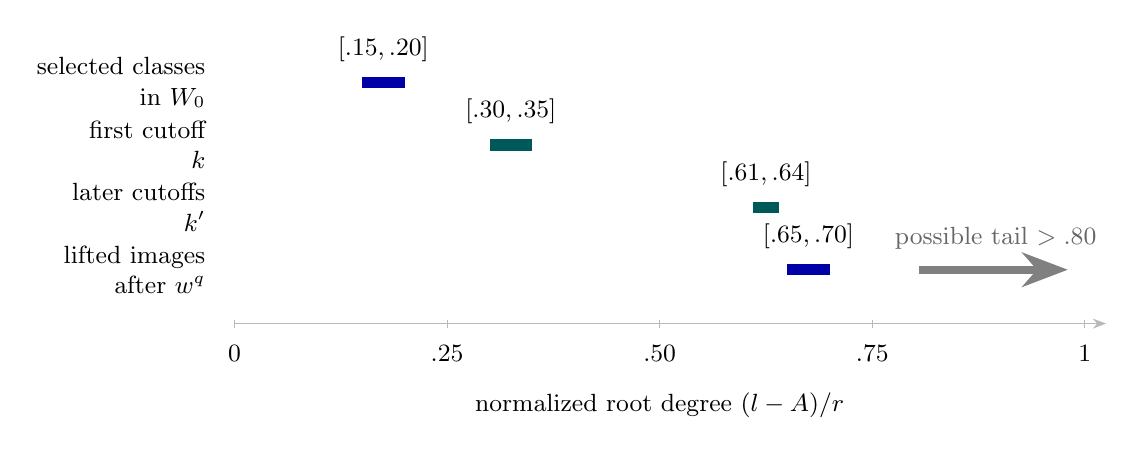
\begin{tikzpicture}[x=10.8cm,y=.72cm,>=Stealth,
  every node/.style={font=\small},
  selected/.style={blue!65!black,line width=4pt},
  cutoff/.style={teal!70!black,line width=4pt},
  remainder/.style={gray,line width=3pt}]
  \draw[gray!55,->] (0,-.65) -- (1.025,-.65);
  \foreach \x/\lab in {0/0,.25/{.25},.5/{.50},.75/{.75},1/1} {
    \draw[gray!55] (\x,-.72) -- (\x,-.58);
    \node[below=3pt] at (\x,-.72) {$\lab$};
  }
  \node[below=20pt] at (.5,-.72) {normalized root degree $(l-A)/r$};

  \node[left=7pt,align=right] at (0,3.6) {selected classes\\in $W_0$};
  \draw[selected] (.15,3.6) -- (.20,3.6);
  \node[above=4pt] at (.175,3.6) {$[.15,.20]$};

  \node[left=7pt,align=right] at (0,2.5) {first cutoff\\$k$};
  \draw[cutoff] (.30,2.5) -- (.35,2.5);
  \node[above=4pt] at (.325,2.5) {$[.30,.35]$};

  \node[left=7pt,align=right] at (0,1.4) {later cutoffs\\$k'$};
  \draw[cutoff] (.61,1.4) -- (.64,1.4);
  \node[above=4pt] at (.625,1.4) {$[.61,.64]$};

  \node[left=7pt,align=right] at (0,.3) {lifted images\\after $w^q$};
  \draw[selected] (.65,.3) -- (.70,.3);
  \node[above=4pt] at (.675,.3) {$[.65,.70]$};
  \draw[remainder,->] (.805,.3) -- (.98,.3);
  \node[above=4pt,text=gray!80!black] at (.895,.3) {possible tail $>.80$};
\end{tikzpicture}
\caption{The degree intervals in Lemma~\ref{trans:no-interior}, normalized
by the gap width $r$; the drawing suppresses rounding errors of order
$r^{-1}$. Multiplication by $w^q$, with $q/r\approx .50$, moves the
selected root degrees above every later cutoff $k'$ while keeping them
separate from the other terms. Multiplication by $v$ then raises actual
degree without changing root labels; the inequality
$2k+q<2k'$ provides the required degree room.}
\label{fig:degree-gap}
\end{figure}

The classes
\[
 v^{\,2k'-(2k+q)}w^q u_\mu
       \in H_K^{2k'}(X_{2a},M)
\]
have unchanged normalized fixed images: multiplication by $v$ changes
the actual degree and leaves the root coefficients unchanged.
Multiplication by $w$ raises each root label by one, as used above.
Thus the images are independent and lie entirely above root cutoff
$k'$, proving
\[
 H_{k',2k'}\ge c_1r
 \quad\text{for every integer }k'\in[A+0.61r,A+0.64r].
\]
There are at least $c_2r$ such cutoffs for large $r$.  The left side of
\eqref{trans:used-budget} is therefore at least
$c_1c_2r^2\ge c_1c_2\delta^2a^2$, contradicting its linear upper bound.
This proves the assertion for the chosen gap.  The finite number of
gaps allows one common lower threshold for $a$.
\end{proof}

\subsection{Bounding the remaining degrees}

\begin{proof}[Proof of Theorem~\ref{thm:bounded-transients}]
First let $a$ be large with $2a$ regular.  By
Lemma~\ref{trans:no-interior}, transient classes can occur only within
distance $c$ of one of the finitely many degrees $s_i a$.
Lemma~\ref{trans:degree-gaps} excludes degrees above the last such
band.  Thus only a bounded number of integer degrees can contribute.
We now bound the dimension in each of them uniformly.

For high degrees, the reflection local ranks of
Theorem~\ref{thm:local-control} give
\begin{equation}\label{trans:high-ranks}
 \dim B_a^j
 \le C\sum_i\#\{m\ge1:m\ell_i<a,\ |j-m\Delta_i|\le C_{\rm loc}+n\}.
\end{equation}
This follows by summing the crossing exact-sequence bounds, starting
with the zero relative group below the first event.
If $\Delta_i>0$, the number in braces is bounded by
$1+2(C_{\rm loc}+n)/\Delta_i$, up to an integer rounding constant.
If $\Delta_i=0$, it is zero once $j>C_{\rm loc}+n$.
The finite prime list therefore gives a uniform bound on
$\dim B_a^j$ in every sufficiently high degree.

The fixed low-degree interval needs a different argument, which also
accounts for all zero-mean-index iterates.  Choose a regular
$a_+\in(a+D,a+D+1)$.  By ordinary death,
\begin{equation}\label{trans:kernel-window}
 \ker\bigl(H_j(X_a,M)\to H_j(\Lambda,M)\bigr)
 =\ker\bigl(H_j(X_a,M)\to H_j(X_{a_+},M)\bigr).
\end{equation}
The kernel on the right is bounded in dimension by the sum of local
ordinary ranks in this interval of cut values of width at most $D+1$.  The number
of its events is at most
\[
 \sum_i\left(2+\frac{D+1}{\ell_i}\right),
\]
independently of $a$.  Uniform local ranks bound the kernel, and the
global-image rank is bounded by the fixed global degree rank.
Consequently $\dim H^j(X_a,M)$ is bounded uniformly in $a$ for each
fixed low degree $j$.

The sign-line Gysin sequence gives
\[
 \dim B_a^j\le\dim B_a^{j-1}+\dim H^j(X_a,M),
 \qquad B_a^{-1}=0.
\]
Induction, including degree zero, bounds $B_a^j$ uniformly throughout
any fixed low-degree interval.  Combining this with
\eqref{trans:high-ranks}, every degree in the finitely many remaining
bands has uniformly bounded dimension.  Since the number of such
degrees is also bounded, their sum bounds $T(a)$ as asserted.

Cuts $a$ in a bounded interval have only finitely many crossing stages,
so they satisfy a common bound as well.  Finally, if $a$ is regular but
$2a$ is not, choose a nearby $a'$ in the same no-critical interval such
that $2a'$ is regular.  The critical values and their halves are locally
finite.  The no-critical restriction isomorphism between the root
sublevels is natural with respect to global restriction, and hence
preserves both $B_a$ and its global image.  In particular
$T(a)=T(a')$.  This proves \eqref{trans:total-bound} for every positive
regular cut.
\end{proof}

We have bounded the total excess dimension at each regular cut without
assuming monotonicity as the cut varies.  The next section proves
monotonicity under doubling.  Together, these statements will force an
interval of maximal transient dimension on which the activation of a
new global class is incompatible with the local evaluation-cup relation.

\section{Doubling and the first activation}\label{sec:activation}

Theorem~\ref{thm:bounded-transients} bounds the total number of reflection
classes which do not come from the whole loop space. We now compare that
number at a cut and its double. Equality in this comparison will require
each visible odd-stage bottom class to have a visible evaluation-cup
partner. At the first appearance of such a bottom, local evaluation
vanishing prevents its partner from appearing. This gives the final
contradiction.

Retain the finite-prime assumption and write
\[
 V(a)=\sum_j\rank(B_\infty^j\longrightarrow B_a^j),
 \qquad
 T(a)=\sum_j\dim B_a^j-V(a).
\]
Both sums are finite at a regular cut. We first record the full-group
rank calculation that makes the doubling comparison exact.

\begin{lemma}[Free rank and torsion at a finite cut]\label{act:module-rank}
Suppose that $2L>0$ is regular, and put
$H=\bigoplus_j H_G^j(X_{2L},M)$. This is a finitely generated graded
$\kk[U]$-module. Its torsion submodule $\mathcal T$ is finite-dimensional
and annihilated by a power of $U$. If
\[
 t=\dim(\mathcal T/U\mathcal T)=\dim\ker(U|_H),
 \qquad \rho=\rank_{\kk[U]}(H/\mathcal T),
\]
then
\begin{equation}\label{act:total-rank}
 \sum_j\dim B_{2L}^j=\rho+2t,
 \qquad \rho=\sum_j\dim B_L^j.
\end{equation}
\end{lemma}

\begin{proof}
The standard-plane Gysin sequence in Proposition~\ref{prop:gysin}
embeds $H/UH$ into $\bigoplus_j B_{2L}^j$, which has finite dimension.
Lift a finite homogeneous basis of $H/UH$. These lifts generate $H$:
subtract their contributions modulo $U$, divide the remainder by $U$,
and induct down the nonnegative degree. This is an induction decreasing
degree by two at each step.

If a polynomial $p(U)$ has nonzero constant term, it acts injectively
on $H$. Indeed, the lowest nonzero homogeneous component of a nonzero
element survives in its product with $p(U)$. Factoring an annihilating
polynomial as $U^s p(U)$ therefore shows that every torsion element is
killed by a power of $U$. The ring $\kk[U]$ is Noetherian, so $\mathcal T$
has finitely many generators and is killed by one common power of $U$.
It is consequently finite-dimensional. Rank-nullity on $\mathcal T$
gives
\[
 \dim\ker(U|_H)=\dim\ker(U|_{\mathcal T})
 =\dim(\mathcal T/U\mathcal T).
\]
Moreover $UH\cap\mathcal T=U\mathcal T$, since $Uh$ torsion implies
that $h$ is torsion.

Set $\mathcal F=H/\mathcal T$. Multiplication by $U$ is injective on
$\mathcal F$. Lift a homogeneous basis of $\mathcal F/U\mathcal F$.
Degree induction again proves generation. These lifts are free: in a
homogeneous relation cancel the least power of $U$ and reduce modulo
$U$. Independence of the selected basis excludes the terms with that
least power, a contradiction. Thus $\mathcal F$ has a homogeneous free
basis of size $\rho$, and
\[
 \dim(H/UH)=\rho+t.
\]
Summing the standard-plane Gysin sequence over degrees gives the first
identity in \eqref{act:total-rank}, since its two contributions are
$H/UH$ and a shifted copy of $\ker U$.

For sufficiently large $D$, the torsion no longer contributes in
degrees $D,D-1$. The dimensions of those two free degrees add to
$\rho$, one contribution from each free generator according to parity.
The weight-two-plane Gysin sequence gives
\[
 \rho=\dim H_G^D(X_{2L},M)+\dim H_G^{D-1}(X_{2L},M)
 =\dim H_K^D(X_{2L},M).
\]
By Lemma~\ref{bud:localization} and \eqref{bud:fixed-product}, the last
dimension equals $\sum_j\dim B_L^j$ in high degree. This proves the
second identity without requiring surjectivity of full-group restriction
to the fixed locus.
\end{proof}

Use the global basis from Theorem~\ref{thm:global-generators}:
\[
 \xi_{m,k}=w^kX_m,\qquad \eta_{m,k}=e\xi_{m,k},
 \qquad m\ge1,\quad 0\le k\le d.
\]
At a regular cut $a$, let $b_{m,k}(a)$ be one if $\xi_{m,k}$ restricts
nontrivially and zero otherwise. Let $h_{m,k}(a)$ be one if the
restriction of $\eta_{m,k}$ is independent modulo all bottom
restrictions in its degree, and zero otherwise. Degrees within the
bottom family are distinct, as are degrees within the top family:
their consecutive starting degrees differ by $2d$, while each family
at a stage spans an interval of width $d$. Therefore
\begin{equation}\label{act:visibility-count}
 V(a)=\sum_{m,k}\bigl(b_{m,k}(a)+h_{m,k}(a)\bigr),
 \qquad h_{m,k}(a)\le b_{m,k}(a).
\end{equation}
The inequality follows from $\eta_{m,k}=e\xi_{m,k}$. Write $V_o(a)$
and $V_e(a)$ for the contributions of odd and even stages $m$ to this
sum. Stage parity here refers to the round-filtration label $m$.

\begin{theorem}[Doubling and its equality condition]\label{thm:doubling}
For every regular $2L>0$,
\begin{equation}\label{act:doubling}
 T(2L)\ge T(L).
\end{equation}
If equality holds, then
\begin{equation}\label{act:odd-equality}
 h_{m,k}(2L)=b_{m,k}(2L)
 \qquad(m\ \text{odd},\ 0\le k\le d).
\end{equation}
\end{theorem}

\begin{proof}
Use the notation of Lemma~\ref{act:module-rank}, and put
\[
 N=\sum_{m\ \mathrm{odd},k} b_{m,k}(2L).
\]
The selected odd bottoms have global $G$-equivariant $U$-torsion lifts
by Theorem~\ref{thm:global-generators}. Their restrictions to $H/UH$
are independent, since that quotient injects into reflection cohomology
and their bottom restrictions are independent. They thus occupy an
$N$-dimensional subspace of $\mathcal T/U\mathcal T$. Write
\begin{equation}\label{act:residual-torsion}
 t=N+J_0,\qquad J_0\ge0.
\end{equation}

The selected even bottoms and tops also have global full-group lifts.
Their classes modulo $U$ are jointly independent with the selected odd
bottoms: this follows from their reflection restrictions and the rule
that a top is counted only modulo all bottoms in its degree. In the
projection
\[
 H/UH\longrightarrow\mathcal F/U\mathcal F,
\]
the kernel is $\mathcal T/U\mathcal T$, of dimension $N+J_0$.
The odd span already occupies $N$ of these dimensions. Hence the image
of the even span has dimension at least $V_e(2L)-J_0$.

Choose a maximal homogeneous independent family among these even
projections; its size is at least $V_e(2L)-J_0$.
Multiply the corresponding global lifts by powers of $U$ to put them in
two common large degrees $D,D-1$, according to parity. Independence persists in
$\mathcal F$: from a relation in one of the common degrees, cancel
the least power of $U$ and reduce modulo $U$, then repeat if necessary.
Thus the sum of the ambient full-group global-image ranks in these
two degrees is at least $V_e(2L)-J_0$.

We compare these images with the fixed locus, including the image-level
Gysin maps. The subspace $X_{2L}^\tau$ is $G$-invariant. Under its
identification with $X_L$, rotations act with doubled parameter and
reflection acts as before. In sufficiently high degree the map
\[
 H_G^q(X_{2L},M)\longrightarrow H_G^q(X_{2L}^\tau,M)
\]
is injective. Indeed, compose it with the injective fixed $G$-to-$K$
restriction. The same composite factors through the ambient
$G$-to-$K$ injection and the high actual $K$ restriction isomorphism
of Lemma~\ref{bud:localization}.

For $H'=G,K$, set
\[
 I_{H'}^q=\im\bigl[H_{H'}^q(\Lambda^\tau,M)
       \longrightarrow H_{H'}^q(X_{2L}^\tau,M)\bigr].
\]
Naturality places the ambient global images inside these fixed global
images. Apply the weight-two-plane Gysin sequence to the fixed global
and fixed finite pairs. Its global push is surjective, so on images
the finite push gives a surjection
\[
 \pi:I_K^D\longrightarrow I_G^{D-1}.
\]
The finite $G$-to-$K$ injection identifies $I_G^D$ with a subspace of
$\ker\pi$. Consequently
\[
 \dim I_G^D+\dim I_G^{D-1}\le\dim I_K^D.
\]
On the fixed $K$-spaces the global restriction is the coefficientwise
map $B_\infty[v]\to B_L[v]$. Since $B_L$ has finite total dimension,
$\dim I_K^D=V(L)$ for sufficiently large $D$. Choose $D$ large enough
for all the preceding comparisons. We have proved
\begin{equation}\label{act:image-inequality}
 V(L)\ge V_e(2L)-J_0.
\end{equation}

Subtract global-image dimensions from \eqref{act:total-rank} and use
\eqref{act:residual-torsion}--\eqref{act:image-inequality}:
\begin{align*}
 T(2L)-T(L)
 &=2(N+J_0)-V_o(2L)-V_e(2L)+V(L)\\
 &\ge J_0+2N-V_o(2L)\\
 &=J_0+\sum_{m\ \mathrm{odd},k}
       \bigl(b_{m,k}(2L)-h_{m,k}(2L)\bigr)\ge0.
\end{align*}
All summands in the final line are nonnegative. Equality therefore
forces \eqref{act:odd-equality} for each individual odd bottom.
\end{proof}

\begin{proof}[Completion of the proof of Theorem~\ref{thm:spheres} for $n\ge3$]
Suppose that there are only finitely many prime geodesic images.
By Theorem~\ref{thm:bounded-transients}, $T$ is a bounded nonnegative
integer on regular positive cuts. It is constant on every no-critical
interval, so its maximum is attained on a nonempty bounded open regular
interval $I\subset(0,\infty)$.

Every regular point $x\in2^kI$ has regular successive halves: a critical
half would double to a critical point. Iterating \eqref{act:doubling}
therefore gives $T(x)\ge T(x/2^k)$, which is already the global maximum.
Thus every regular point in every expanded interval attains that maximum.
For $k\ge1$, equality holds between $x$ and $x/2$, so
\eqref{act:odd-equality} holds at every such $x$. This uses monotonicity
under doubling only; no monotonicity between arbitrary cuts is asserted.

Take $k$ large and choose regular $x_1<x_2$ in the lower and upper
quarters of $2^kI$. The interval of degrees strictly between
$\alpha x_1$ and $\alpha x_2$, after removing the fixed endpoint margins
of Lemma~\ref{trans:degree-gaps}, has length tending to infinity.
Remove also the fixed-width bands about every $\beta_i x_1$ and
$\beta_i x_2$. They remove a bounded total number of possible degrees.
The odd bottom degrees
\[
 a_m=(2m-1)d,\qquad m\ \text{odd},
\]
form an arithmetic progression of spacing $4d$. For sufficiently large
$k$, one such degree $j=a_m$ remains, beyond the fixed low-degree range.
Lemma~\ref{trans:degree-gaps} makes $\xi_{m,0}$ invisible at $x_1$
and visible at $x_2$. At $x_1$ the degree lies in an absent gap, where
the global image is zero, or above the last band, where the sublevel
group is zero. At $x_2$ it lies in a present gap where global reflection
restriction is injective.

A global class nonzero at a smaller sublevel cannot become zero at a
larger one, since restriction to the smaller sublevel factors through
the larger. There are only finitely many events between $x_1$ and $x_2$.
Choose the first event at which $\xi_{m,0}$ becomes nonzero, and tight
regular cuts $x_-<x_+$ around it, still inside $2^kI$. The exact sequence
of the crossing puts its post-event restriction in the image of
\[
 H_R^j(X_{x_+},X_{x_-})\longrightarrow B_{x_+}^j,
\]
because its pre-event restriction is zero. By
Theorem~\ref{thm:local-control}, cup with $e$ vanishes on this whole
reflection crossing, including simultaneous prime labels. Naturality
of the cup action therefore gives
\[
 \eta_{m,0}|_{X_{x_+}}=e\,\xi_{m,0}|_{X_{x_+}}=0.
\]
Hence $b_{m,0}(x_+)=1$ while $h_{m,0}(x_+)=0$. Since $m$ is odd,
this contradicts \eqref{act:odd-equality} at the regular point $x_+$
of the expanded interval. The finite-prime-image assumption is impossible.
\end{proof}

\section{Finite spherical covers}\label{sec:covers}
\begin{proof}[Proof of Corollary~\ref{cor:finite-cover}]
Let $\pi:\widetilde M\to M$ be a finite smooth covering of degree $r$,
where $\widetilde M$ is diffeomorphic to $S^n$.  Equip $\widetilde M$
with the pullback of the given metric.  The map $\pi$ is then a local
isometry, so it sends every nonconstant closed geodesic upstairs to a
nonconstant closed geodesic downstairs.  Taking the least positive
period of the latter does not change its image.

We show that at most $r$ upstairs prime images project to any one
downstairs prime image.  Choose an oriented unit-speed representative
$\sigma:\mathbb R\to M$ of that image, of least period $L>0$, and
put $p=\sigma(0)$.  For each $q\in\pi^{-1}(p)$ there is a unique lift
of $\sigma$ starting at $q$, with initial velocity
$(\dd\pi_q)^{-1}\dot\sigma(0)$.  Lifting one period permutes the finite
fiber $\pi^{-1}(p)$; lifting the reversed path gives the inverse
permutation.  After $m\le r$ periods a lift therefore returns to its
initial point.  Its velocity also returns, because the downstairs
velocity returns and $\dd\pi_q$ is invertible.  The lift is a closed
geodesic.  If $m$ is the first return of that fiber point, its least
period is $mL$: any period upstairs projects to a period of $\sigma$
and hence is an integer multiple of $L$.

By Lemma~\ref{lem:local-prime-images}, unit-speed geodesics with the
same image agree after a parameter shift and possibly reversal.
Consequently any upstairs prime geodesic whose projected image is the
chosen one can be parametrized so that its projection is exactly
$\sigma$.  It is then one of the lifts starting at the $r$ points
above $p$.  This proves the finite-fiber bound.  The argument permits
self-intersections and does not require the covering to be regular;
phase or reversal can only identify some of these finitely many images.

Theorem~\ref{thm:spheres} gives infinitely many upstairs prime images
for the pullback metric.  Since every downstairs prime image has at
most $r$ preimages in this set, there are infinitely many downstairs
prime images as well.
\end{proof}

\bibliographystyle{plain}
\bibliography{references}
\end{document}
